% review_panel_slides.tex -- presentation of analysis documents v1.6 to the review panel.
% Main slides follow the logic of analysis_note.tex and proton_tagged_note.tex; the backup slides carry the
% main material of technical_supplement.tex. Every number is taken from the v1.6 documents (tag v1.6).
% Build: pdflatex review_panel_slides (twice).
\documentclass[aspectratio=169,10pt]{beamer}
\usepackage{graphicx}
\usepackage{booktabs}
\usepackage{amsmath}
\usepackage{tikz}
\usetikzlibrary{arrows.meta,positioning}
\graphicspath{{figures/}}

\definecolor{ubred}{RGB}{160,20,20}
\definecolor{ubdark}{RGB}{90,10,10}
\definecolor{ublight}{RGB}{205,70,70}
\usetheme{default}
\setbeamercolor{structure}{fg=ubred}
\setbeamercolor{title}{fg=ubdark}
\setbeamercolor{frametitle}{fg=white,bg=ubred}
\setbeamercolor{section in head/foot}{fg=white,bg=ubdark}
\setbeamercolor{alerted text}{fg=ubred}
\setbeamercolor{block title}{fg=white,bg=ubred}
\setbeamercolor{block body}{bg=ubred!8}
\setbeamercolor{itemize item}{fg=ubred}
\setbeamercolor{itemize subitem}{fg=ublight}
\setbeamertemplate{navigation symbols}{}
\setbeamertemplate{frametitle}{\vskip4pt\usebeamercolor[fg]{frametitle}%
  \begin{beamercolorbox}[wd=\paperwidth,ht=2.4ex,dp=1ex,leftskip=.3cm]{frametitle}%
  \bfseries\insertframetitle\end{beamercolorbox}}

% Main frames are numbered n / N; backup frames B1, B2, ...
\newif\ifbackup
\setbeamertemplate{footline}{%
  \leavevmode\hbox{%
  \begin{beamercolorbox}[wd=.62\paperwidth,ht=2.4ex,dp=1ex,leftskip=.3cm]{section in head/foot}%
  \usebeamerfont{author in head/foot}\insertshortauthor\ | MicroBooNE NuMI CC$\pi^{\pm}$ | v1.6\hfill\end{beamercolorbox}%
  \begin{beamercolorbox}[wd=.38\paperwidth,ht=2.4ex,dp=1ex,rightskip=.3cm]{section in head/foot}%
  \hfill\insertshorttitle\quad\ifbackup Backup \insertframenumber\else\insertframenumber\,/\,\pageref{mainend}\fi\end{beamercolorbox}}}

% Every result figure is from pseudo-data; the stamp is drawn by LaTeX, as in the notes.
\newcommand{\blindfig}[2][\textwidth]{%
  \begin{tikzpicture}
    \node[inner sep=0pt] (img) {\includegraphics[width=#1]{#2}};
    \node[anchor=north east, fill=red!12, draw=red!60!black, rounded corners=1pt, inner sep=1.5pt,
          font=\tiny\bfseries\sffamily, text=red!60!black] at ([xshift=-2pt,yshift=-2pt]img.north east)
          {BLINDED: CV PSEUDO-DATA};
  \end{tikzpicture}}
\newcommand{\blindfigh}[2][\textheight]{%
  \begin{tikzpicture}
    \node[inner sep=0pt] (img) {\includegraphics[height=#1]{#2}};
    \node[anchor=north east, fill=red!12, draw=red!60!black, rounded corners=1pt, inner sep=1.5pt,
          font=\tiny\bfseries\sffamily, text=red!60!black] at ([xshift=-2pt,yshift=-2pt]img.north east)
          {BLINDED: CV PSEUDO-DATA};
  \end{tikzpicture}}
\newcommand{\GeVc}{\,\text{GeV}/c}
\newcommand{\src}[1]{\par\vfill\hfill{\tiny\color{gray}#1}}

\title[Review panel]{Differential CC$\pi^{\pm}$ cross sections on argon in the NuMI beam}
\subtitle{$\nu_\mu+\bar\nu_\mu$, FHC, RHC and combined; inclusive and proton-tagged}
\author[Pophale, Nowak]{Ishanee Pophale and Jarek Nowak}
\institute{Lancaster University}
\date{Review panel, 30 September 2026\\[1mm]\footnotesize Analysis documents v1.6 (tag \texttt{v1.6}, 34baa99)}

\begin{document}

{\setbeamertemplate{footline}{}
\begin{frame}[plain]
  \titlepage
  \begin{center}\footnotesize\color{ubdark}
  The signal region is blind. Every cross section shown is extracted from central-value pseudo-data.
  \end{center}
\end{frame}}

% =====================================================================
\begin{frame}{The documents and this talk}
  \begin{columns}[T]
  \column{.5\textwidth}
  \textbf{Three documents (v1.6)}
  \begin{itemize}\small
    \item \textbf{Analysis note} (54\,pp.): measurement definition, selection, extraction, uncertainties,
      validation, inclusive results.
    \item \textbf{Proton-tagged note} (18\,pp.): subsample with a reconstructed proton above
      $0.3\GeVc$; refers to the analysis note for everything shared.
    \item \textbf{Technical supplement} (54\,pp.): final configuration, evidence for each choice,
      rejected alternatives.
    \item Data release: $A_C$, covariances by source and curves of $59$ extractions.
  \end{itemize}
  \column{.5\textwidth}
  \textbf{Outline} (order of the analysis note)
  \begin{enumerate}\small\setlength\itemsep{0pt}
    \item Measurement definition
    \item Beam, flux, exposure, samples
    \item Signal definition and selection
    \item Backgrounds and control regions
    \item Extraction: response, binning, Wiener-SVD
    \item Systematic uncertainties
    \item Validation
    \item Inclusive results
    \item Proton-tagged subsample
    \item Limitations and summary
  \end{enumerate}
  Backup: technical supplement.
  \end{columns}
\end{frame}

% =====================================================================
\section{Measurement definition}
\begin{frame}{Measurement definition}
  \centering\scriptsize\setlength{\tabcolsep}{4pt}
  \begin{tabular}{@{}p{2.6cm}p{11.6cm}@{}}
    \toprule
    Interaction & $\nu_\mu$ or $\bar\nu_\mu$ CC on argon; $\mu^-\pi^+$ and $\mu^+\pi^-$ both signal (charge-blind) \\
    Final state & Exactly one $\mu$ and one $\pi^\pm$ among primaries; no $\pi^0$, kaon or other meson; any number of nucleons; coherent included \\
    Phase space & $p_\mu>0.15\GeVc$, $p_\pi>0.175\GeVc$, $\theta_{\mu\pi}<2.6$\,rad \\
    Vertex & True vertex in FV $10<x<246$, $-101<y<101$, $10<z<986$\,cm, excluding $675.1<z<775.1$\,cm \\
    Neutrino direction & Angles about the $\nu$: true direction per event (truth), NuMI target$\to$vertex (reco), $28.6^\circ$ from detector $z$ \\
    Flux & $\Phi_{\nu_\mu}+\Phi_{\bar\nu_\mu}$, new-G4 PPFX CV, $E_\nu>60$\,MeV: FHC $6.81159$, RHC $6.44646$, comb.\ $6.59691\times10^{-10}$\,cm$^{-2}$POT$^{-1}$ \\
    Exposure & FHC $7.766$, RHC $11.082$, combined $18.848\times10^{20}$\,POT; each run normalised to its own exposure \\
    Target & $N_\mathrm{Ar}=8.710\times10^{29}$ argon nuclei in the FV \\
    Normalisation & $10^{-38}$\,cm$^2$/Ar;\; $d\sigma/dx|_j=\hat N_j/(\Delta x_j\,\Phi\,N_\mathrm{Ar})$ \\
    Unfolding & Wiener-SVD; result estimates $A_C\,x_\mathrm{true}$; predictions compared after $A_C$; one-bin total has $A_C=1$ \\
    Observables & $p_\mu$ (6), $p_\pi$ (3 regions), $\cos\theta_\mu$ (8), $\cos\theta_\pi$ (5), $\theta_{\mu\pi}$ (5), one-bin total; FHC, RHC, comb.\\
     & $\cos\theta_\pi\times\cos\theta_\mu$ ($2\times3$), combined only \\
    Covariance & Flux, interaction model, re-interaction, detector, $\mu$ momentum scale, POT, targets, MC/EXT/data statistics \\
    \bottomrule
  \end{tabular}
  \vspace{2mm}
  \begin{columns}[T]
  \column{.48\textwidth}\scriptsize
  \textbf{Primary results}: 15 differential extractions (5 observables $\times$ 3 configurations) and 3 one-bin totals.
  \column{.48\textwidth}\scriptsize
  \textbf{Secondary result}: $d^2\sigma/d\cos\theta_\pi\,d\cos\theta_\mu$, combined. Proton-tagged results in the companion note.
  \end{columns}
\end{frame}

\begin{frame}{Physics context}
  \begin{columns}[T]
  \column{.52\textwidth}
  \begin{itemize}\small\setlength\itemsep{3pt}
    \item CC$\pi^\pm$ is among the most frequent interactions at $1$--$5$\,GeV and a background to
      $\nu_e$ appearance (NOvA, T2K, DUNE).
    \item Dominated by $\Delta(1232)$; non-resonant + DIS $\approx20\%$; coherent $\le10\%$ (signal).
    \item FSI (absorption $25$--$30\%$, charge exchange) moves events between CC$\pi^\pm$, CC$\pi^0$,
      CC$0\pi$ at the $30\%$ level: the signal is defined by the final state.
    \item Response and pseudo-data from the MicroBooNE tune of GENIE v3.
    \item Standalone generators span a factor $1.6$ in the total, GENIE lowest, NEUT highest.
  \end{itemize}
  \column{.46\textwidth}
  \scriptsize\setlength{\tabcolsep}{2pt}
  \begin{tabular}{@{}p{1.3cm}p{2.1cm}p{2.9cm}@{}}
    \toprule
    Generator & Resonances & FSI \\\midrule
    GENIE v3 & KLN--BS, 18 res. & INTRANUKE hA \\
    NuWro & $\Delta$ only & Salcedo--Oset cascade \\
    NEUT & mod.\ R--S, 18 res. & step-by-step cascade \\
    GiBUU & in-medium spectral fn. & transport, $\pi$ optical pot. \\
    \bottomrule
  \end{tabular}\\[3mm]
  \textbf{Closest measurements}
  \begin{itemize}\scriptsize
    \item MicroBooNE BNB CC$1\pi^\pm$: $\sigma=(3.75\pm0.80)\times10^{-38}$\,cm$^2$/Ar, $\langle E\rangle\approx0.7$\,GeV.
    \item MicroBooNE NuMI $\nu_e$ CC$\pi^+$: same beam, framework and conventions.
    \item The value here, $\approx1.0\times10^{-38}$, is not directly comparable to BNB: the flux
      average runs from $60$\,MeV while pion production starts near $0.3$\,GeV.
  \end{itemize}
  \end{columns}
\end{frame}

% =====================================================================
\section{Beam, flux and exposure}
\begin{frame}{NuMI flux and exposure}
  \begin{columns}[T]
  \column{.47\textwidth}
  \scriptsize\centering\setlength{\tabcolsep}{3pt}
  \textbf{Integrated flux} ($10^{-10}$\,cm$^{-2}$POT$^{-1}$, $E_\nu>60$\,MeV)\\[1mm]
  \begin{tabular}{lcccc}
    \toprule
    & $\Phi_{\nu_\mu}$ & $\Phi_{\bar\nu_\mu}$ & $\Phi_{\nu_\mu+\bar\nu_\mu}$ & $\bar\nu_\mu$ \\\midrule
    FHC & $4.43515$ & $2.37644$ & $6.81159$ & $34.9\%$ \\
    RHC & $2.92348$ & $3.52298$ & $6.44646$ & $54.6\%$ \\
    Comb. & $3.54634$ & $3.05057$ & $6.59691$ & $46.2\%$ \\
    \bottomrule
  \end{tabular}\\[2mm]
  \begin{itemize}\scriptsize\setlength\itemsep{1pt}
    \item Each configuration normalised with its own flux (RHC is $5.4\%$ below FHC).
    \item Mean energy $0.48$\,GeV; only $40\%$ of the flux lies above $0.3$\,GeV.
    \item PPFX CV weight on every event (mean $0.944$ on selected signal); flux integrals validated
      four ways.
    \item Selected RHC events are $76\%$ $\nu_\mu$: the $\nu_\mu$ cross section is 2--3$\times$ larger.
  \end{itemize}
  \column{.5\textwidth}
  \scriptsize\centering\setlength{\tabcolsep}{4pt}
  \textbf{Exposure by run} ($10^{20}$\,POT)\\[1mm]
  \begin{tabular}{lccc}
    \toprule
    Run & MC POT & Data POT & Scale \\\midrule
    Run 1 FHC & 23.282 & 2.192 & 0.0942 \\
    Run 2 FHC & 24.934 & 1.268 & 0.0509 \\
    Run 4 FHC & 28.335 & 2.075 & 0.0732 \\
    Run 5 FHC & 19.300 & 2.231 & 0.1156 \\
    \textbf{FHC} & \textbf{95.85} & \textbf{7.766} & per run \\\midrule
    Run 1 RHC & 8.997 & 0.605 & 0.0673 \\
    Run 2 RHC & 57.865 & 2.591 & 0.0448 \\
    Run 3 RHC & 55.185 & 5.003 & 0.0907 \\
    Run 4 RHC & 32.586 & 2.883 & 0.0885 \\
    \textbf{RHC} & \textbf{154.63} & \textbf{11.082} & per run \\\midrule
    \textbf{Combined} & \textbf{250.49} & \textbf{18.848} & per run \\
    \bottomrule
  \end{tabular}\\[1mm]
  \raggedright FHC Run 1 is the non-open-trigger data: $2.192\times10^{20}$\,POT, $5\,748\,692$ triggers (runs 4952--6748).
  Pseudo-data are thrown run by run at each run's exposure.
  \end{columns}
\end{frame}

\begin{frame}{Beam direction in detector coordinates}
  \centering
  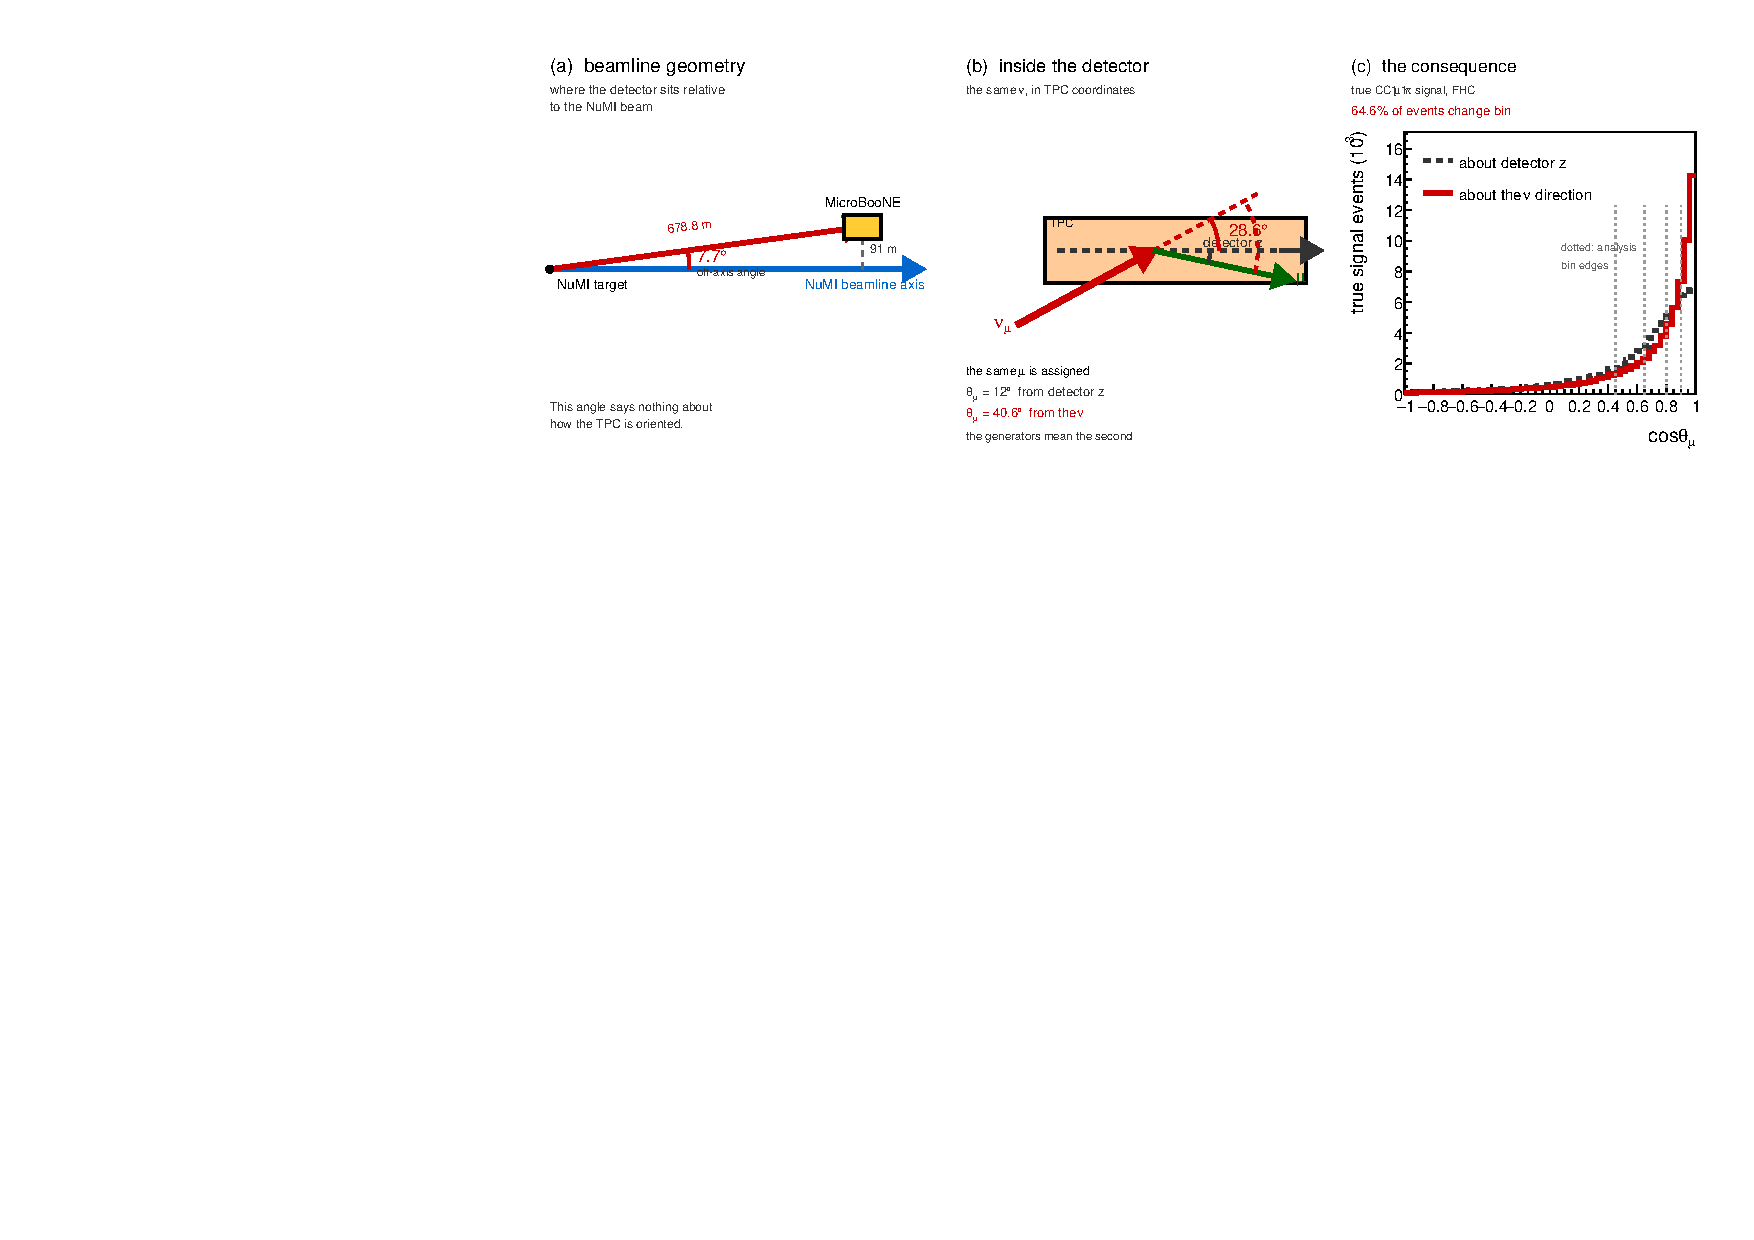
\includegraphics[width=0.94\textwidth]{numi_geometry}
  \begin{columns}[T]
  \column{.49\textwidth}
  \begin{itemize}\scriptsize\setlength\itemsep{2pt}
    \item Off-axis angle $7.71^\circ$ ($134.6$\,mrad): property of the beamline.
    \item Neutrinos arrive $28.6^\circ$ from detector $z$ (mean true direction $(0.462,0.049,0.885)$).
    \item Generators use $\theta$ about the $\nu$; about $z$, $64.6\%$ of events change
      $\cos\theta_\mu$ bin ($44.6\%$ for $\cos\theta_\pi$).
  \end{itemize}
  \column{.49\textwidth}
  \begin{itemize}\scriptsize\setlength\itemsep{2pt}
    \item Truth: per-event $\nu$ direction. Reco: NuMI target to reconstructed vertex ($\beta$ convention
      of the NuMI $\nu_e$ CC$1\pi$ analysis).
    \item Fixed axis vs.\ per-event $\beta$: median $2.4$\,mrad, $0.42\%$ of muons change bin.
    \item Momenta, $\theta_{\mu\pi}$, $W_{\pi p}$, totals and the selection do not depend on the axis.
  \end{itemize}
  \end{columns}
\end{frame}

\begin{frame}{Samples, event weights and beam-off normalisation}
  \begin{columns}[T]
  \column{.5\textwidth}
  \scriptsize\setlength{\tabcolsep}{2pt}
  \begin{tabular}{@{}p{2.2cm}p{3.9cm}c@{}}
    \toprule
    Sample & Composition & $n$ \\\midrule
    $\nu_\mu$ overlay FHC & Runs 1, 2, 4 + Run 5 (rew.\ PPFX) & 4 \\
    $\nu_\mu$ overlay RHC & Runs 1, 2, 3, 4a, 4b, 4c & 10 \\
    Dirt & GENIE NuMI dirt per run and mode & 7 \\
    EXT (beam-off) & cosmic data per run, mode-independent & 7 \\
    Detector var. & Run-4 FHC + RHC, CV + 8 knobs & 18 \\
    Pseudo-data & Poisson-thrown CV, per run & \\
    \bottomrule
  \end{tabular}\\[2mm]
  \textbf{Weight}\; $w=\text{Scale[run]}\times w_\mathrm{PPFX}\times w_\mathrm{tune}$,\;
  set to 1 if non-finite, negative or $>30$. The same rule in universes, covariance, cut-flow, control
  regions and the beam-on comparison.
  \column{.48\textwidth}
  \scriptsize
  \textbf{Beam-off (EXT)}
  \[\text{EXT}_\text{run}=0.98\,\frac{\text{triggers}_\text{on}[\text{run}]}{\sum_\text{files}\text{triggers}_\text{off}}\sum_\text{files}N^\text{sel}_\text{EXT}\]
  \begin{itemize}\setlength\itemsep{1pt}
    \item Matched by run period, independent of horn polarity.
    \item No Run-2 beam-off: Run 1 used (both pre-CRT).
    \item Selected rate per $10^6$ triggers: 1.75 (R1), 0.43 (R3b), 1.15 (R4), 0.52 (R5).
    \item At the final cut: 23 (FHC), 23 (RHC), 46 (comb.) events, $1.3$--$1.6\%$ of the sample.
    \item No extra cosmic cut: a data-driven subtraction of $\approx5$ events' uncertainty; every variant removes more signal.
  \end{itemize}
  \end{columns}
\end{frame}

% =====================================================================
\section{Signal and selection}
\begin{frame}{Signal definition and the pion threshold}
  \begin{columns}[T]
  \column{.48\textwidth}
  \begin{itemize}\small\setlength\itemsep{3pt}
    \item Generator level; used for efficiency and response, never as a reco cut.
    \item $|\nu_\mathrm{PDG}|=14$, CC, true vertex in FV.
    \item Exactly one $\mu$ and one $\pi^\pm$ (any momentum); a second $\pi^\pm$ below threshold makes the event background.
    \item Thresholds set by the efficiency turn-on ($10$\,cm $\mu$, $20$\,cm $\pi$ track length).
    \item $\theta_{\mu\pi}<2.6$\,rad removes a region of $\approx7\%$ purity (cosmic, dirt); applied at reco too.
  \end{itemize}
  \column{.5\textwidth}
  \scriptsize\centering
  \textbf{Pion momentum reconstruction vs.\ true $p_\pi$}\\[1mm]
  \setlength{\tabcolsep}{3pt}
  \begin{tabular}{lccc}
    \toprule
    True $p_\pi$ [GeV/$c$] & Bias & RMS & Reco frac. \\\midrule
    0.080--0.113 & $+131\%$ & $73\%$ & $3.4\%$ \\
    0.113--0.150 & $+66\%$ & $56\%$ & $3.4\%$ \\
    0.150--0.175 & $+30\%$ & $51\%$ & $4.3\%$ \\
    \textbf{0.175--0.250} & $\mathbf{-8\%}$ & $\mathbf{31\%}$ & $\mathbf{10.0\%}$ \\
    0.250--0.400 & $-30\%$ & $21\%$ & $10.4\%$ \\
    \bottomrule
  \end{tabular}\\[2mm]
  \raggedright
  The NuMI $\nu_e$ analysis uses KE$_\pi>40$\,MeV ($p_\pi>0.113$). Below $0.175\GeVc$ the few
  reconstructed pions are those long enough to pass, biased up; resolution $51$--$56\%$,
  efficiency $2.2\%$. No cross section is reported below $0.175\GeVc$.
  \end{columns}
\end{frame}

\begin{frame}{Event selection}
  \begin{columns}[T]
  \column{.52\textwidth}
  \scriptsize
  \begin{enumerate}\setlength\itemsep{0pt}
    \item[1.] \textbf{NeutrinoSlice}: $\ge1$ track, software trigger
    \item[2.] \textbf{InFiducialVol}: SCE-corrected reco vertex in FV
    \item[3.] \textbf{Topological} score $>0.67$ (EXT down $\times28$--$29$)
    \item[4.] \textbf{MuonCandidate}: track score $>0.8$, $d_\mathrm{vtx}\le4$\,cm, $L>10$\,cm, LLR $>0.2$, MIP BDT $\ge-0.1$; highest muon-BDT score
    \item[5.] \textbf{ContainedPion}: exactly one other track with track score $\ge0.5$, LLR $>0.1$, $L>20$\,cm, MIP BDT $>-0.1$, pion BDT $>-0.1$, Bragg-$\pi$ $\ge0.08$, end contained
    \item[6--7.] \textbf{$\mu$, $\pi$ in 3 planes}
    \item[8.] \textbf{ShowerCut}: no primary shower, except one small shower ($<50$ Y hits, $>10$\,cm)
    \item[9.] \textbf{OpeningAngle} $\theta_{\mu\pi}<2.6$\,rad
    \item[10.] \textbf{Nonprotons}: $<4$ tracks with LLR $>0.1$, $<5$ tracks
  \end{enumerate}
  BDTs (TMVA) use Bragg likelihoods, LLR, track score and end points; the candidate-PID BDTs do not use
  track length, so they do not sculpt the momentum spectra.
  \column{.46\textwidth}
  \scriptsize\centering
  \textbf{Kinematics}
  \begin{itemize}\raggedright\setlength\itemsep{2pt}
    \item $p_\mu$: range if contained ($37\%$), MCS if exiting ($63\%$); MCS bias $-10\%$, resolution $30\%$.
    \item $p_\pi$: range under $\mu$ hypothesis, converted to $\pi$ at fixed KE in the bin definition
      (lowest bin reco/true $0.888\to0.976$).
    \item Angles about $\hat u_\nu$; $\theta_{\mu\pi}$ from track directions only.
  \end{itemize}
  \vspace{2mm}
  \setlength{\tabcolsep}{3pt}
  \begin{tabular}{lcc}
    \toprule
    Final cut & Efficiency & Purity \\\midrule
    FHC & $17.5\%$ & $58.5\%$ \\
    RHC & $17.6\%$ & $57.4\%$ \\
    Combined & $17.6\%$ & $57.9\%$ \\
    \bottomrule
  \end{tabular}
  \end{columns}
\end{frame}

\begin{frame}{Cut-flow at full exposure}
  \begin{columns}[T]
  \column{.56\textwidth}
  \scriptsize\setlength{\tabcolsep}{2.5pt}\centering
  FHC, $7.766\times10^{20}$\,POT (CV weight, per-run scaling)\\[1mm]
  \begin{tabular}{lrrrrrr}
    \toprule
    Cut & Signal & Bkg & EXT & Dirt & Eff\% & Pur\% \\\midrule
    None & 4\,753 & 235\,281 & 3\,256\,689 & 170\,169 & 100.0 & 0.1 \\
    InFiducialVol & 3\,955 & 52\,835 & 122\,860 & 8\,738 & 83.2 & 2.1 \\
    Topological & 2\,995 & 24\,262 & 4\,299 & 827 & 63.0 & 9.2 \\
    MuonCandidate & 2\,689 & 16\,484 & 1\,870 & 530 & 56.6 & 12.5 \\
    ContainedPion & 1\,195 & 1\,823 & 173 & 90 & 25.1 & 36.4 \\
    MuonIn3Planes & 1\,143 & 1\,722 & 144 & 66 & 24.1 & 37.2 \\
    PionIn3Planes & 1\,062 & 1\,549 & 113 & 37 & 22.3 & 38.5 \\
    ShowerCut & 896 & 783 & 83 & 31 & 18.9 & 50.0 \\
    OpeningAngle & 890 & 710 & 32 & 10 & 18.7 & 54.2 \\
    \textbf{Nonprotons} & \textbf{833} & \textbf{560} & \textbf{23} & \textbf{6.6} & \textbf{17.5} & \textbf{58.5} \\
    \bottomrule
  \end{tabular}\\[2mm]
  \begin{tabular}{lrrrrrr}
    \toprule
    Final cut & Signal & Bkg & EXT & Dirt & Eff\% & Pur\% \\\midrule
    RHC & 1\,015 & 720 & 23 & 9.5 & 17.6 & 57.4 \\
    Combined & 1\,848 & 1\,280 & 46 & 16 & 17.6 & 57.9 \\
    \bottomrule
  \end{tabular}
  \column{.42\textwidth}
  \centering
  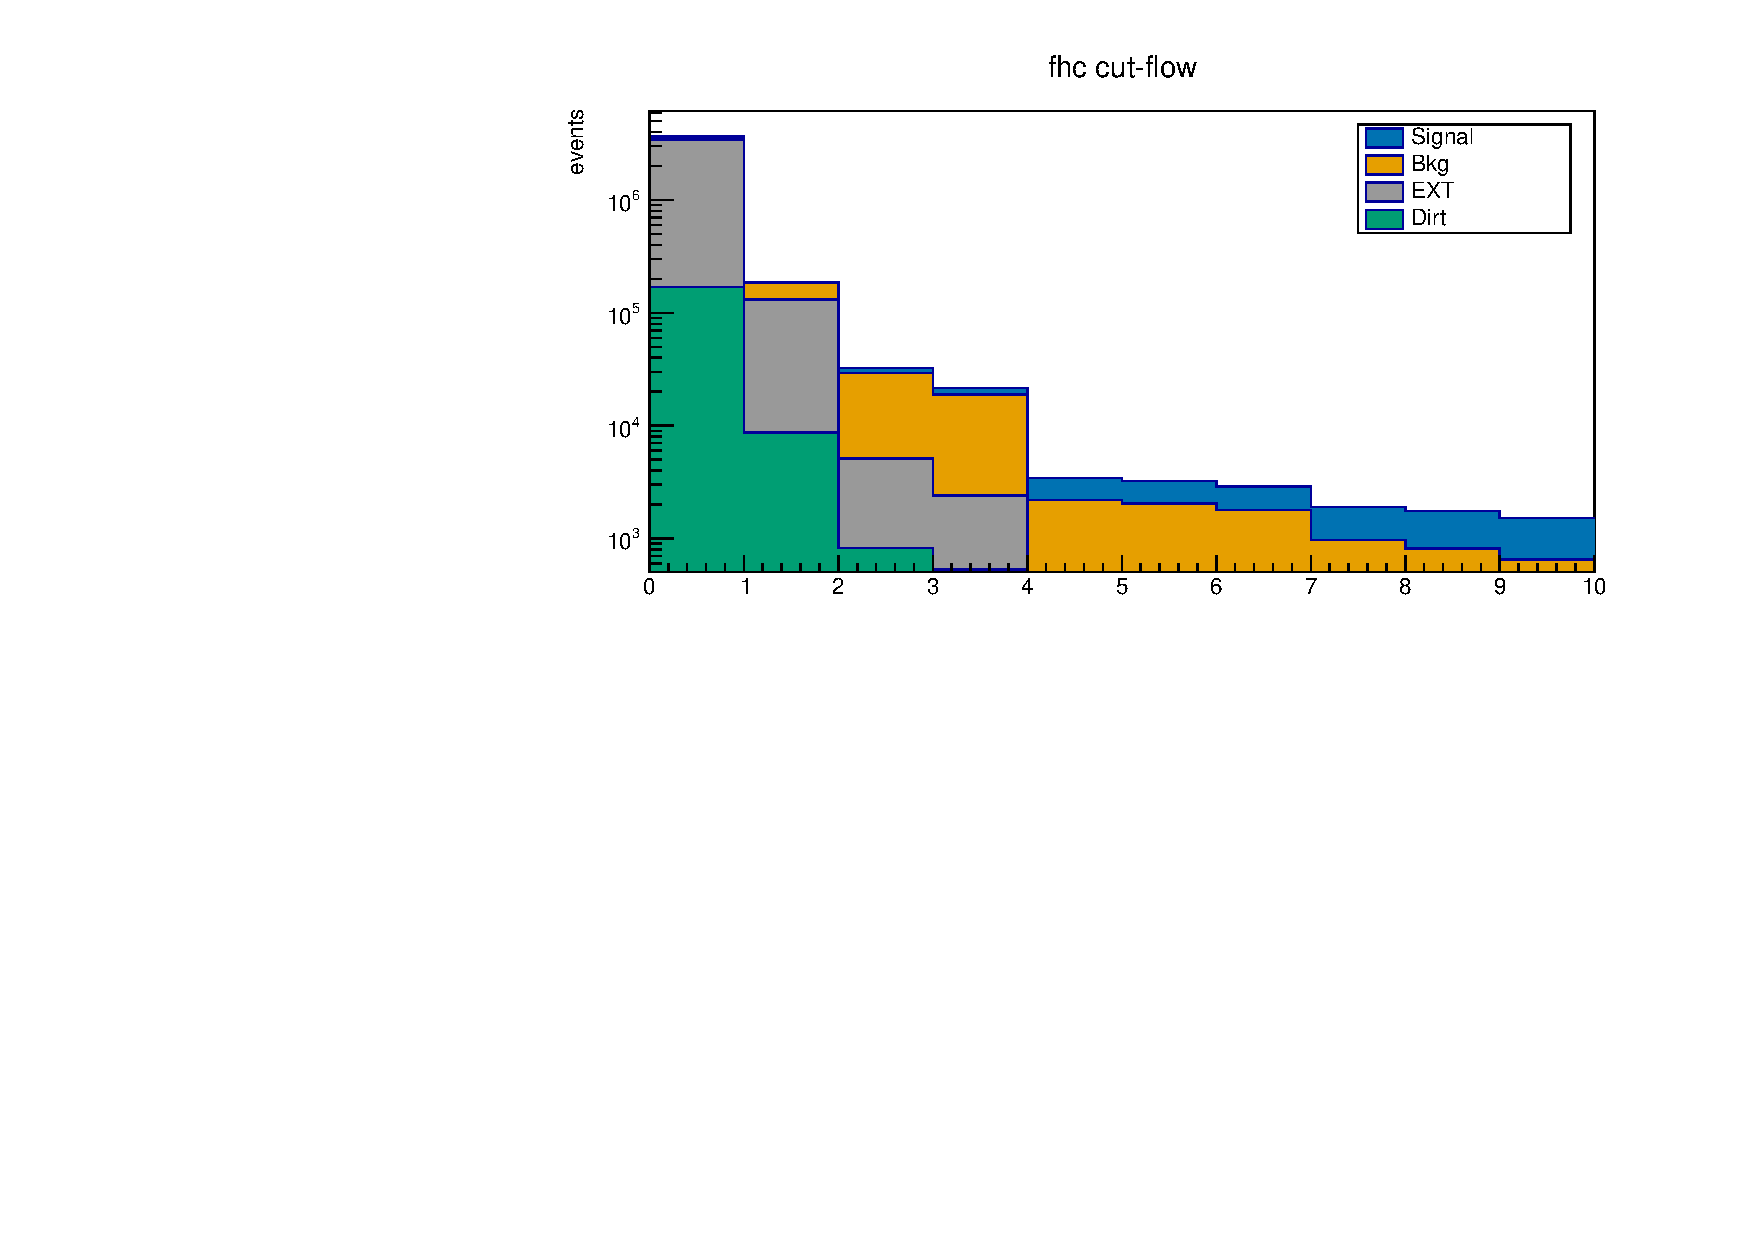
\includegraphics[width=\textwidth]{cutflow_yields_fhc}\\
  {\scriptsize Without the opening-angle cut: purity $54.8\%$, EXT $64$ events.}
  \end{columns}
\end{frame}

% =====================================================================
\section{Backgrounds}
\begin{frame}{Background composition}
  \begin{columns}[T]
  \column{.44\textwidth}
  \scriptsize\centering
  FHC final cut, $560$ neutrino-background events\\[1mm]
  \setlength{\tabcolsep}{3pt}
  \begin{tabular}{lrr}
    \toprule
    Category & Events & Frac. \\\midrule
    CC$0\pi$ (proton or other track as $\pi$) & 215 & $38\%$ \\
    CC $\ge2\pi^\pm$, no $\pi^0$ & 128 & $23\%$ \\
    NC and $\nu_e$CC & 79.0 & $14\%$ \\
    CC with a $\pi^0$ & 51.4 & $9\%$ \\
    CC$1\pi^\pm$ outside phase space & 46.5 & $8\%$ \\
    Out of FV & 41.3 & $7\%$ \\\midrule
    EXT & 23 & \\
    Dirt & 6.6 & \\
    \bottomrule
  \end{tabular}\\[2mm]
  \raggedright
  \begin{itemize}\setlength\itemsep{1pt}
    \item At the working point the pion candidate is a proton in $\approx18\%$ of selected events.
    \item Tighter Bragg-$\pi$ cuts ($0.20$--$0.30$) do not improve the FoM: $\pi:p\approx4:1$ among
      pion candidates in signal, and a tighter cut removes both at similar rates.
  \end{itemize}
  \column{.54\textwidth}
  \centering
  \vspace{4mm}
  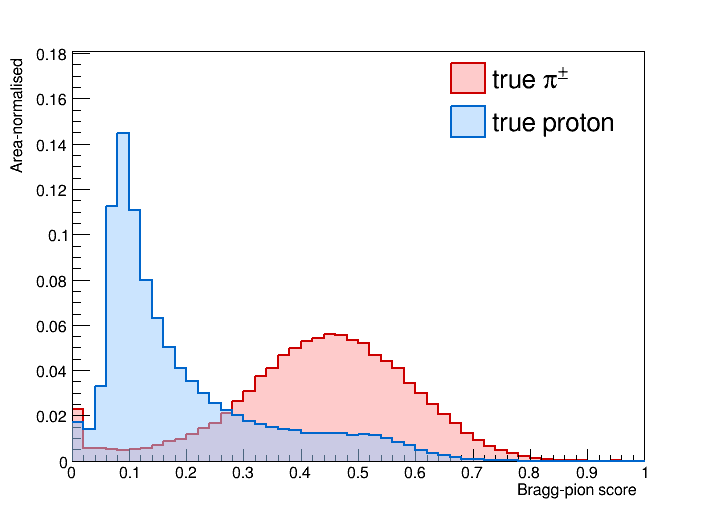
\includegraphics[width=0.85\textwidth]{pid_bpion}\\
{\scriptsize Bragg-$\pi$ score for true $\pi^\pm$ and protons at the final cut; threshold $\ge0.08$.}
  \end{columns}
\end{frame}

\begin{frame}{Background control regions}
  \begin{columns}[T]
  \column{.5\textwidth}
  \centering
  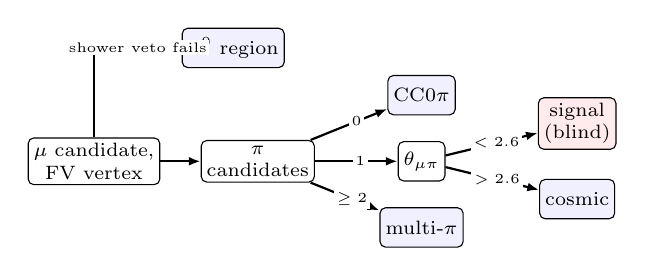
\begin{tikzpicture}[font=\scriptsize, x=0.52mm, y=0.6mm,
      box/.style={draw, rounded corners=2pt, align=center, inner sep=2pt, minimum height=5mm},
      sig/.style={box, fill=red!8}, cr/.style={box, fill=blue!6},
      ar/.style={-{Latex[length=1.5mm]}, thick},
      lbl/.style={font=\tiny, fill=white, inner sep=1pt}]
    \node[box] (pre) at (0,0) {$\mu$ candidate,\\FV vertex};
    \node[cr] (pi0) at (34,24) {$\pi^0$ region};
    \node[box] (np) at (40,0) {$\pi$\\candidates};
    \node[cr] (cc0) at (80,14) {CC$0\pi$};
    \node[cr] (multi) at (80,-14) {multi-$\pi$};
    \node[box] (oa) at (80,0) {$\theta_{\mu\pi}$};
    \node[sig] (sr) at (118,8) {signal\\(blind)};
    \node[cr] (cos) at (118,-8) {cosmic};
    \draw[ar] (pre) -- (np);
    \draw[ar] (pre.north) |- node[lbl, pos=0.75]{shower veto fails} (pi0.west);
    \draw[ar] (np) -- node[lbl, pos=0.6]{$0$} (cc0);
    \draw[ar] (np) -- node[lbl, pos=0.6]{$\ge2$} (multi);
    \draw[ar] (np) -- node[lbl, pos=0.55]{$1$} (oa);
    \draw[ar] (oa) -- node[lbl, pos=0.55]{$<2.6$} (sr);
    \draw[ar] (oa) -- node[lbl, pos=0.55]{$>2.6$} (cos);
  \end{tikzpicture}\\[2mm]
  \raggedright\scriptsize
  \begin{itemize}\setlength\itemsep{1pt}
    \item Each region inverts one requirement; zero events shared with the signal region
      (checked event by event).
    \item CC$0\pi$: dominant background class, $T\approx0.03$, transfer uncertainty $31$--$34\%$ (detector).
    \item $\pi^0$: target CC+NC $\pi^0$, purity $50$--$51\%$, $T\approx0.02$.
    \item multi-$\pi$ and cosmic: diagnostic.
    \item About $30\%$ of the neutrino background has no region of its own.
  \end{itemize}
  \column{.48\textwidth}
  \scriptsize\centering\setlength{\tabcolsep}{2.5pt}
  Expected yields, FHC\\[1mm]
  \begin{tabular}{lrrrrc}
    \toprule
    Region & Signal & $\nu$ bkg & EXT & Dirt & Sig.\ frac. \\\midrule
    CC$0\pi$ & 987 & 9\,703 & 1\,080 & 49 & $9.2\%$ \\
    multi-$\pi$ & 27 & 83 & 5.4 & 0.1 & $24.4\%$ \\
    $\pi^0$ & 582 & 5\,265 & 613 & 10 & $10.0\%$ \\
    cosmic & 5.1 & 60 & 40 & 1.9 & $7.8\%$ \\
    \bottomrule
  \end{tabular}\\[2mm]
  \raggedright
  \begin{itemize}\setlength\itemsep{1pt}
    \item Studied with pseudo-data only: large regions within $1\%$ of unity; full-stack test
      (with EXT and dirt thrown) $0.99$--$1.12$.
    \item The comparison with beam-on data follows a frozen procedure (global $\chi^2$ over 8
      region$\times$mode totals, pulls, shape tests, pre-declared responses), backup.
    \item The control regions contain unselected signal, so they will be opened after approval and before the signal region.
    \item Background-fit toys: pull widths $0.89$--$1.03$.
  \end{itemize}
  \end{columns}
\end{frame}

% =====================================================================
\section{Extraction}
\begin{frame}{Extraction chain}
  \centering
  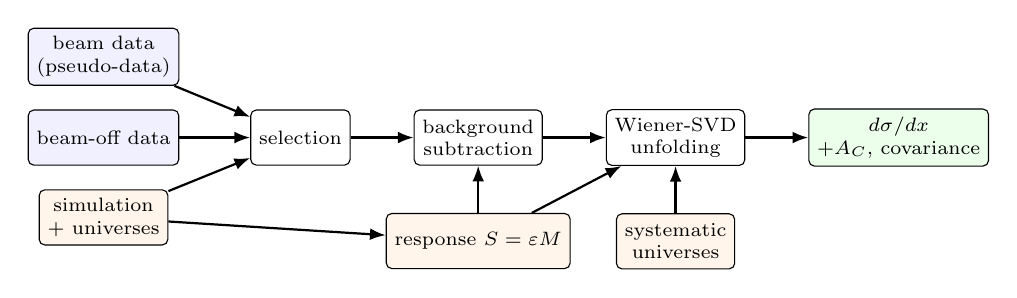
\begin{tikzpicture}[font=\scriptsize,
      box/.style={draw, rounded corners=2pt, align=center, inner sep=3pt, minimum height=7mm},
      data/.style={box, fill=blue!6}, mc/.style={box, fill=orange!8}, res/.style={box, fill=green!8},
      ar/.style={-{Latex[length=2mm]}, thick}]
    \node[data] (d) {beam data\\(pseudo-data)};
    \node[data, below=3mm of d] (ext) {beam-off data};
    \node[mc, below=3mm of ext] (mc) {simulation\\+ universes};
    \node[box, right=9mm of ext] (sel) {selection};
    \node[box, right=8mm of sel] (sub) {background\\subtraction};
    \node[box, right=8mm of sub] (unf) {Wiener-SVD\\unfolding};
    \node[res, right=8mm of unf] (xs) {$d\sigma/dx$\\$+A_C$, covariance};
    \node[mc, below=6mm of sub] (resp) {response $S=\varepsilon M$};
    \node[mc, below=6mm of unf] (cov) {systematic\\universes};
    \draw[ar] (d) -- (sel); \draw[ar] (ext) -- (sel); \draw[ar] (mc) -- (sel);
    \draw[ar] (sel) -- (sub); \draw[ar] (sub) -- (unf); \draw[ar] (unf) -- (xs);
    \draw[ar] (resp) -- (sub); \draw[ar] (resp) -- (unf); \draw[ar] (cov) -- (unf); \draw[ar] (mc) -- (resp);
  \end{tikzpicture}
  \vspace{2mm}
  \begin{columns}[T]
  \column{.5\textwidth}
  \scriptsize
  \vspace{-2mm}
  \begin{align*}
    d^\mathrm{sig}_i&=d^\mathrm{data}_i-b^{\nu}_i-b^\mathrm{EXT}_i-b^\mathrm{dirt}_i\\
    n_i&=\textstyle\sum_j S_{ij}N_j+b_i,\qquad S_{ij}=\varepsilon_jM_{ij}
  \end{align*}
  \begin{itemize}\setlength\itemsep{1pt}
    \item $S$ carries the efficiency, so $\hat N_j$ is efficiency corrected; no separate $1/\varepsilon_j$.
    \item Up to half of a bin comes from other true bins: direct inversion is unstable.
    \item $\mathrm{conv}=N_\mathrm{Ar}\Phi/10^{-38}$: $4608$ (FHC), $6223$ (RHC), $10830$ (comb.).
  \end{itemize}
  \column{.48\textwidth}
  \centering
  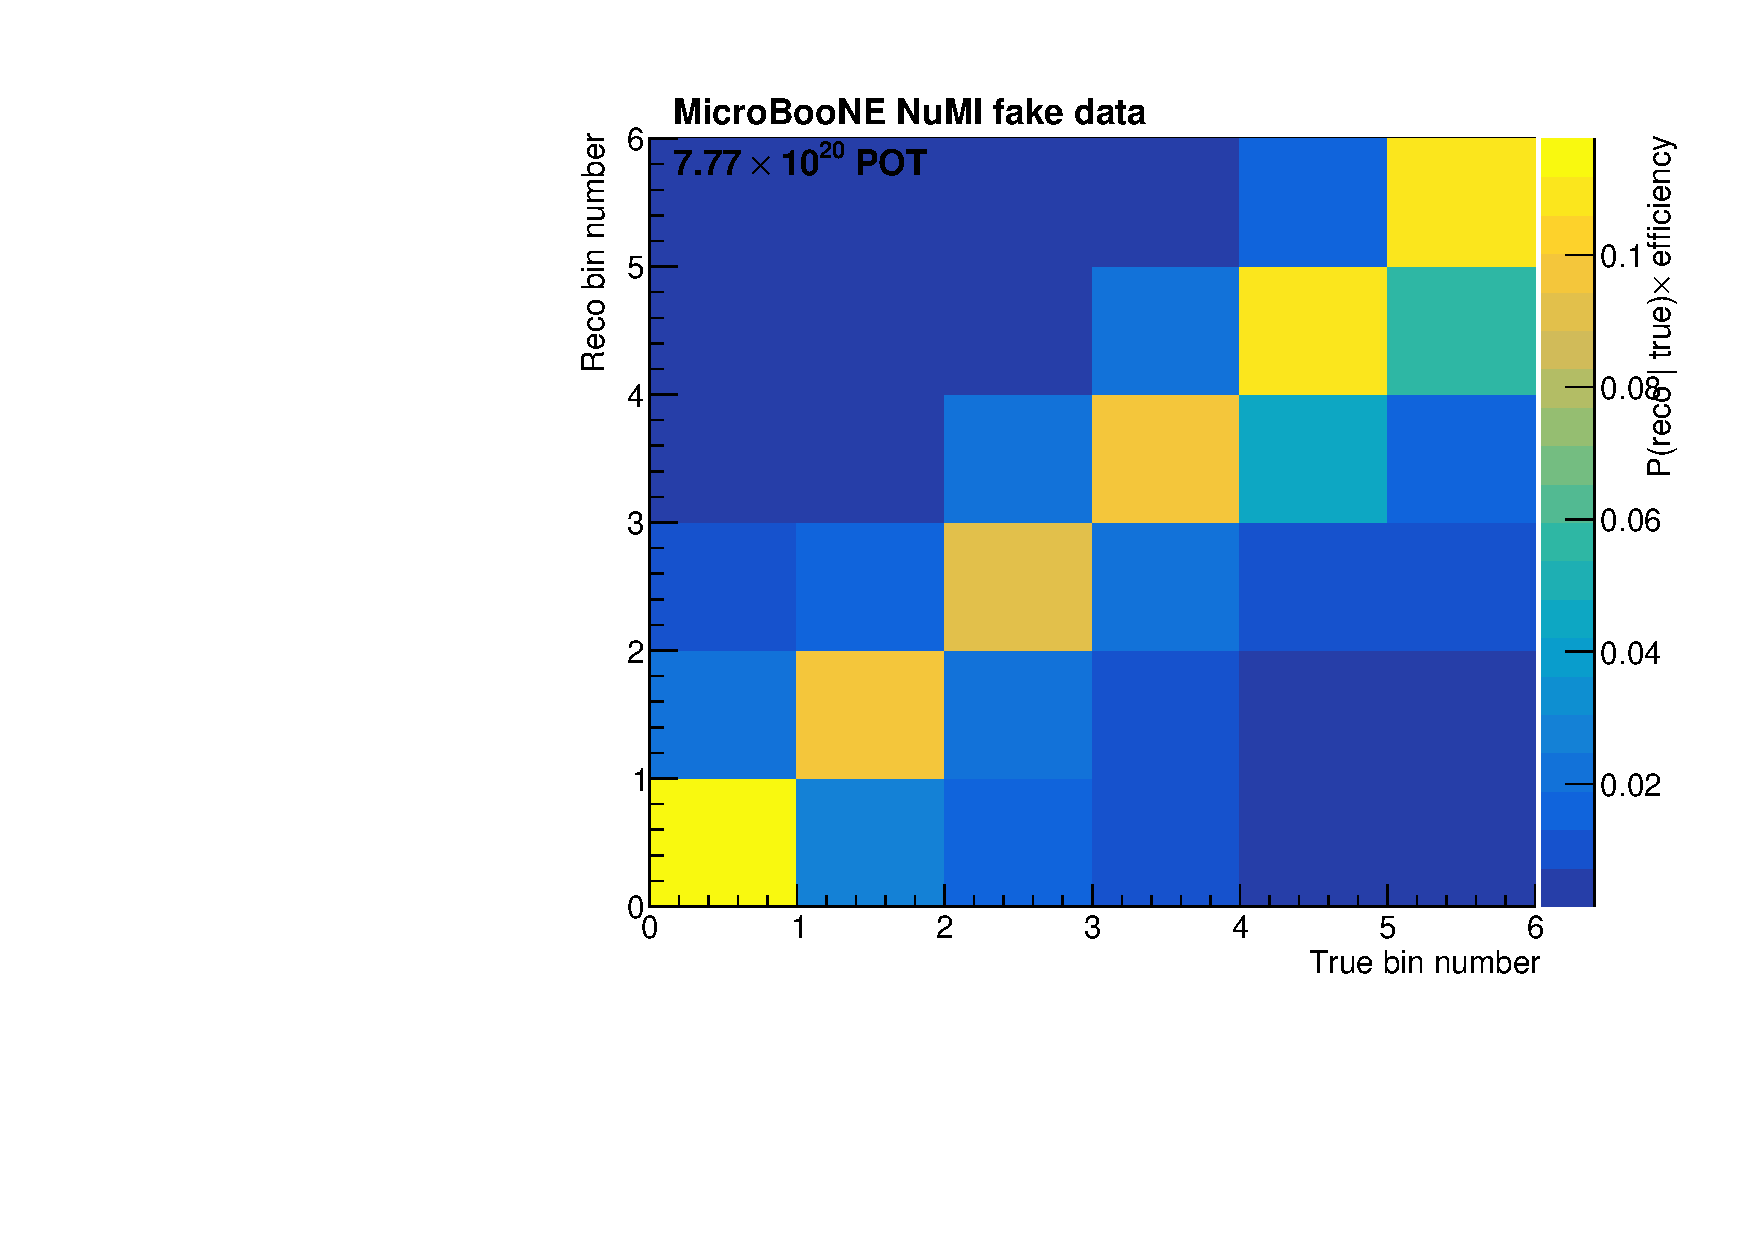
\includegraphics[width=0.49\textwidth]{fw_resp_pmu}\hfill
  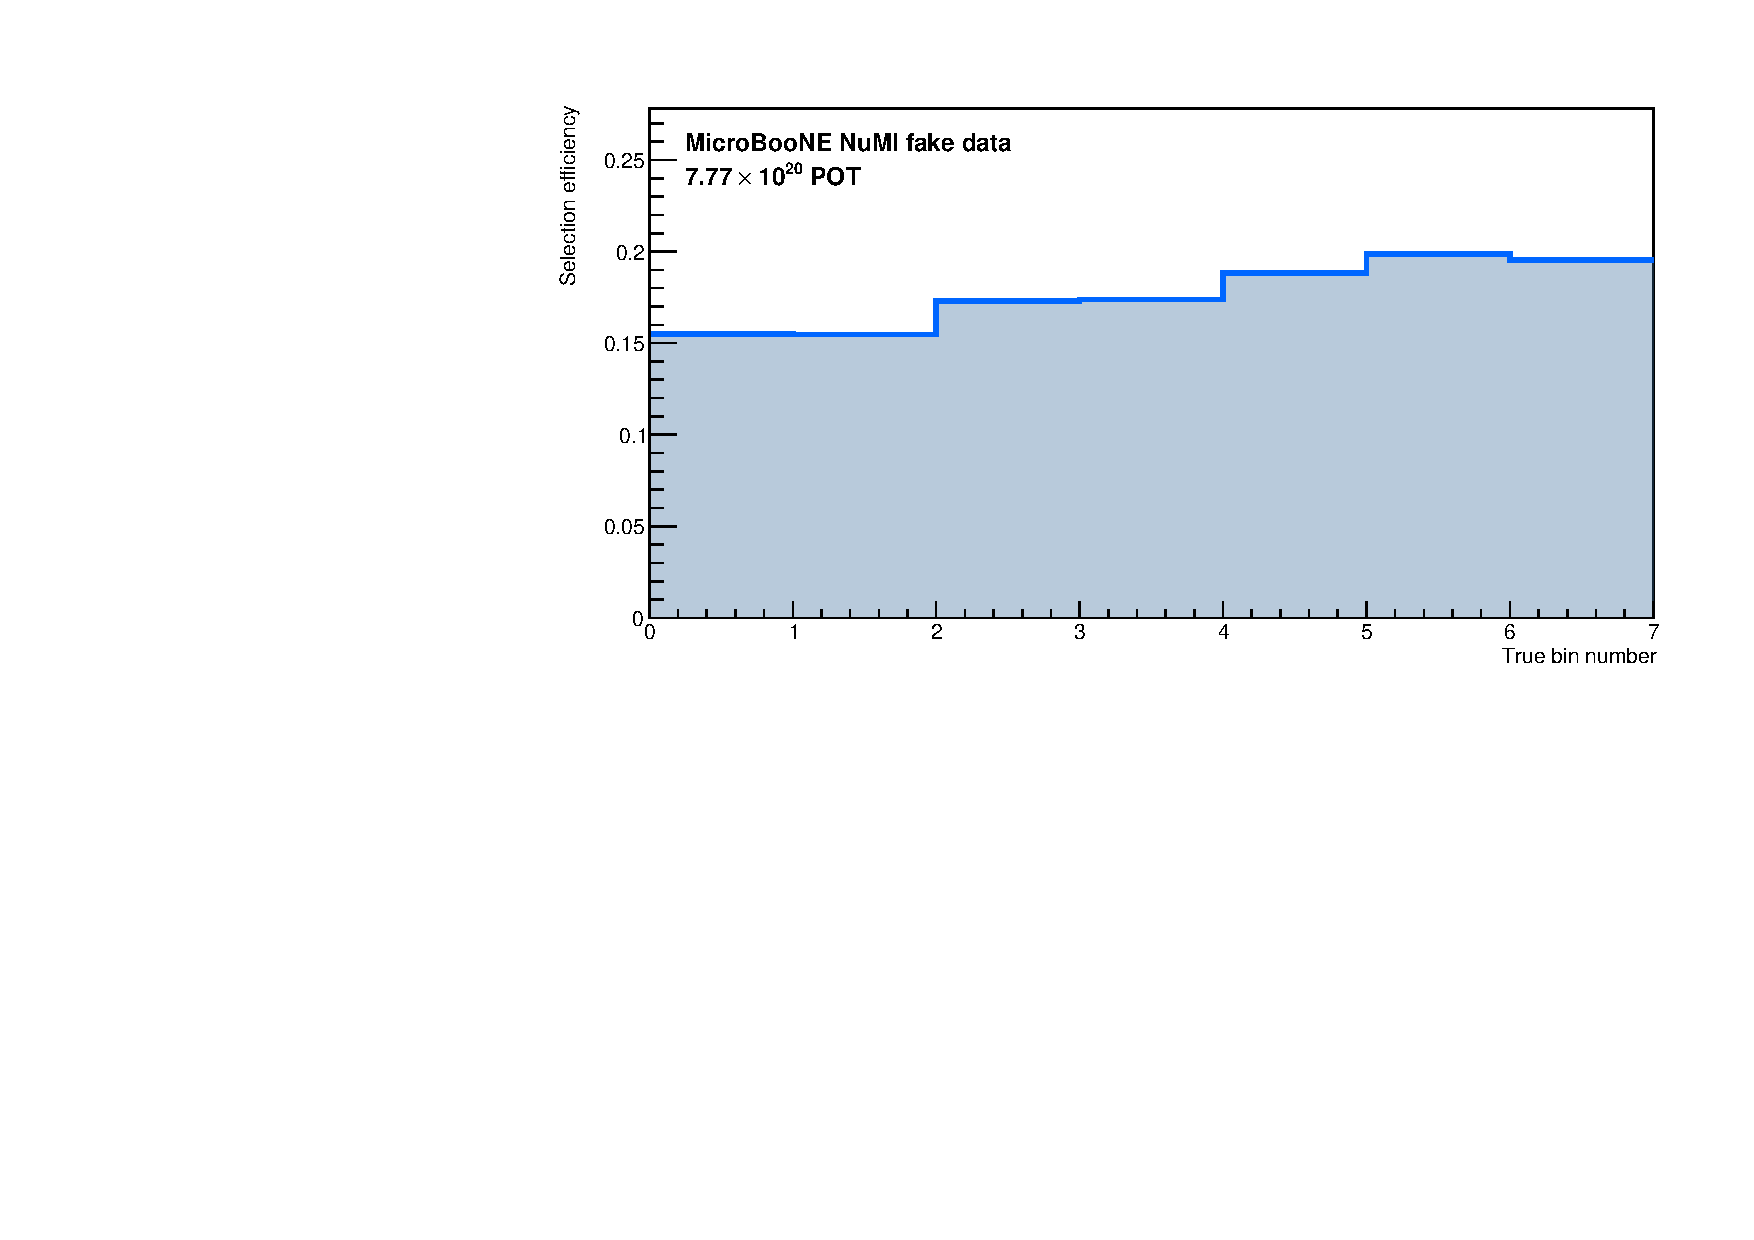
\includegraphics[width=0.49\textwidth]{fw_eff_pmu}\\
  {\scriptsize FHC $p_\mu$: response $S$ (left) and efficiency (right). Efficiency is $13$--$20\%$
  across all observables (the smallest $\theta_{\mu\pi}$ bin $9\%$).}
  \end{columns}
\end{frame}

\begin{frame}{Binning and the migration criterion}
  \begin{columns}[T]
  \column{.47\textwidth}
  \footnotesize
  \begin{itemize}\setlength\itemsep{3pt}
    \item Migration diagonal $M_{jj}$: fraction of selected signal of true bin $j$ reconstructed in bin $j$.
    \item BNB CC$1\pi^\pm$ used $0.68$; here $63\%$ of muons are MCS ($30\%$ resolution) and $p_\pi$ saturates near $0.34\GeVc$.
    \item \textbf{Adopted}: every diagonal $\ge0.50$ in FHC and RHC, $\ge70$ selected signal per bin (50 proton-tagged), fewest bins reaching $90\%$ of the largest trace of $A_C$.
    \item Trace of $A_C$ = degrees of freedom the data determine.
    \item Under $0.68$: $p_\mu$ 4 bins, $p_\pi$ 2 regions, $\cos\theta_\mu$ 7 bins.
    \item The stronger model dependence admitted by $0.50$ is tested by ensembles and reweighted-model pseudo-data.
  \end{itemize}
  \column{.51\textwidth}
  \scriptsize\centering\setlength{\tabcolsep}{2.5pt}
  \textbf{Information content, FHC}\\[1mm]
  \begin{tabular}{lcccccc}
    \toprule
    Observable & bins & min.\ diag. & $A_C$ row sums & tr $A_C$ & $W_k\ge0.5$ & unc. \\\midrule
    $p_\mu$ & 6 & 0.57 & 0.45--0.98 & 2.09 & 2 & $42\%$ \\
    $p_\pi$ & 3 & 0.51 & 0.52--0.91 & 1.57 & 2 & $60\%$ \\
    $\cos\theta_\mu$ & 8 & 0.66 & 0.49--0.70 & 4.00 & 4 & $43\%$ \\
    $\cos\theta_\pi$ & 5 & 0.74 & 0.68--0.78 & 3.11 & 4 & $42\%$ \\
    $\theta_{\mu\pi}$ & 5 & 0.79 & 0.52--1.04 & 2.35 & 3 & $38\%$ \\
    \bottomrule
  \end{tabular}\\[3mm]
  \textbf{Edges}\\[1mm]
  \begin{tabular}{ll}
    \toprule
    $p_\mu$ (GeV/$c$) & 0.15, 0.3, 0.425, 0.575, 0.825, 1.25, open \\
    $p_\pi$ (GeV/$c$) & 0.175, 0.205, 0.26, open \\
    $\cos\theta_\mu$ & $-1$, 0.4, 0.625, 0.75, 0.825, 0.9, 0.95, 0.975, 1 \\
    $\cos\theta_\pi$ & $-1$, $-0.1$, 0.35, 0.6, 0.8, 1 \\
    $\theta_{\mu\pi}$ (rad) & 0, 0.6, 0.85, 1.3, 1.85, 2.6 \\
    \bottomrule
  \end{tabular}
  \end{columns}
\end{frame}

\begin{frame}{Wiener-SVD and the additional-smearing matrix $A_C$}
  \begin{columns}[T]
  \column{.5\textwidth}
  \small
  \begin{itemize}\setlength\itemsep{3pt}
    \item Each SVD mode weighted by $W_k=\sigma_k^2/(\sigma_k^2+N_k)$, set by the data covariance, not tuned by hand.
    \item Regulariser: second derivative of the density with the actual bin widths (widths vary up to
      $56{:}1$); a uniform stencil drives $A_C$ to rank one (backup).
    \item The result estimates $A_C\,x_\mathrm{true}$. Every prediction is smeared by $A_C$ once:
      $\mathrm{smeared}_i=\sum_j (A_C)_{ij}p_j/w_i$.
    \item $A_C$ does not preserve normalisation: integrals differ between observables. The total is taken
      from the one-bin extraction ($A_C\equiv1$).
    \item D'Agostini cross-check: integral flat across observables to $1\%$ and equal to the one-bin total.
  \end{itemize}
  \column{.48\textwidth}
  \scriptsize\centering\setlength{\tabcolsep}{3pt}
  \textbf{$A_C$ row sums}\\[1mm]
  \begin{tabular}{lccc}
    \toprule
    & FHC & RHC & Comb. \\\midrule
    $p_\mu$ & 0.45--0.98 & 0.35--0.72 & 0.45--0.73 \\
    $p_\pi$ & 0.52--0.91 & 0.45--0.89 & 0.45--0.89 \\
    $\cos\theta_\mu$ & 0.49--0.70 & 0.26--0.88 & 0.47--0.67 \\
    $\cos\theta_\pi$ & 0.68--0.78 & 0.70--0.84 & 0.70--0.83 \\
    $\theta_{\mu\pi}$ & 0.52--1.04 & 0.58--1.15 & 0.63--1.20 \\
    \bottomrule
  \end{tabular}\\[3mm]
  \raggedright
  FHC $p_\mu$: smeared/true integral $0.77$--$0.79$ for all four generators, while their true totals
  span $0.82$--$1.32$. The common factor does not create the model differences.\\[2mm]
  Released: curves (already smeared), $A_C$, covariance by source; external reproduction of all $96$
  generator curves to $4\times10^{-8}$.
  \end{columns}
\end{frame}

% =====================================================================
\section{Systematics}
\begin{frame}{Systematic uncertainties}
  \begin{columns}[T]
  \column{.43\textwidth}
  \scriptsize\centering\setlength{\tabcolsep}{3pt}
  Bin-averaged, 15 inclusive differential results\\[1mm]
  \begin{tabular}{llc}
    \toprule
    Source & Method & Range (\%) \\\midrule
    Flux & PPFX, 600 univ. & 22.8--38.5 \\
    Detector & Run-4 var.\ samples & 16.6--34.2 \\
    Cross section & GENIE multisim+unisims & 8.4--16.6 \\
    Re-interaction & Geant4Reweight & 3.5--13.3 \\
    POT & & 2.8--4.5 \\
    Targets & & 1.4--2.2 \\
    MCS scale & data-side $\pm5\%$ & 0.0--10.8 \\\midrule
    MC stat & & 1.9--6.1 \\
    EXT stat & & 0.5--2.3 \\
    Data stat & & 6.6--19.3 \\\midrule
    Prediction total & & 32.6--56.7 \\
    Total & & 33.7--60.0 \\
    \bottomrule
  \end{tabular}
  \column{.55\textwidth}
  \centering
  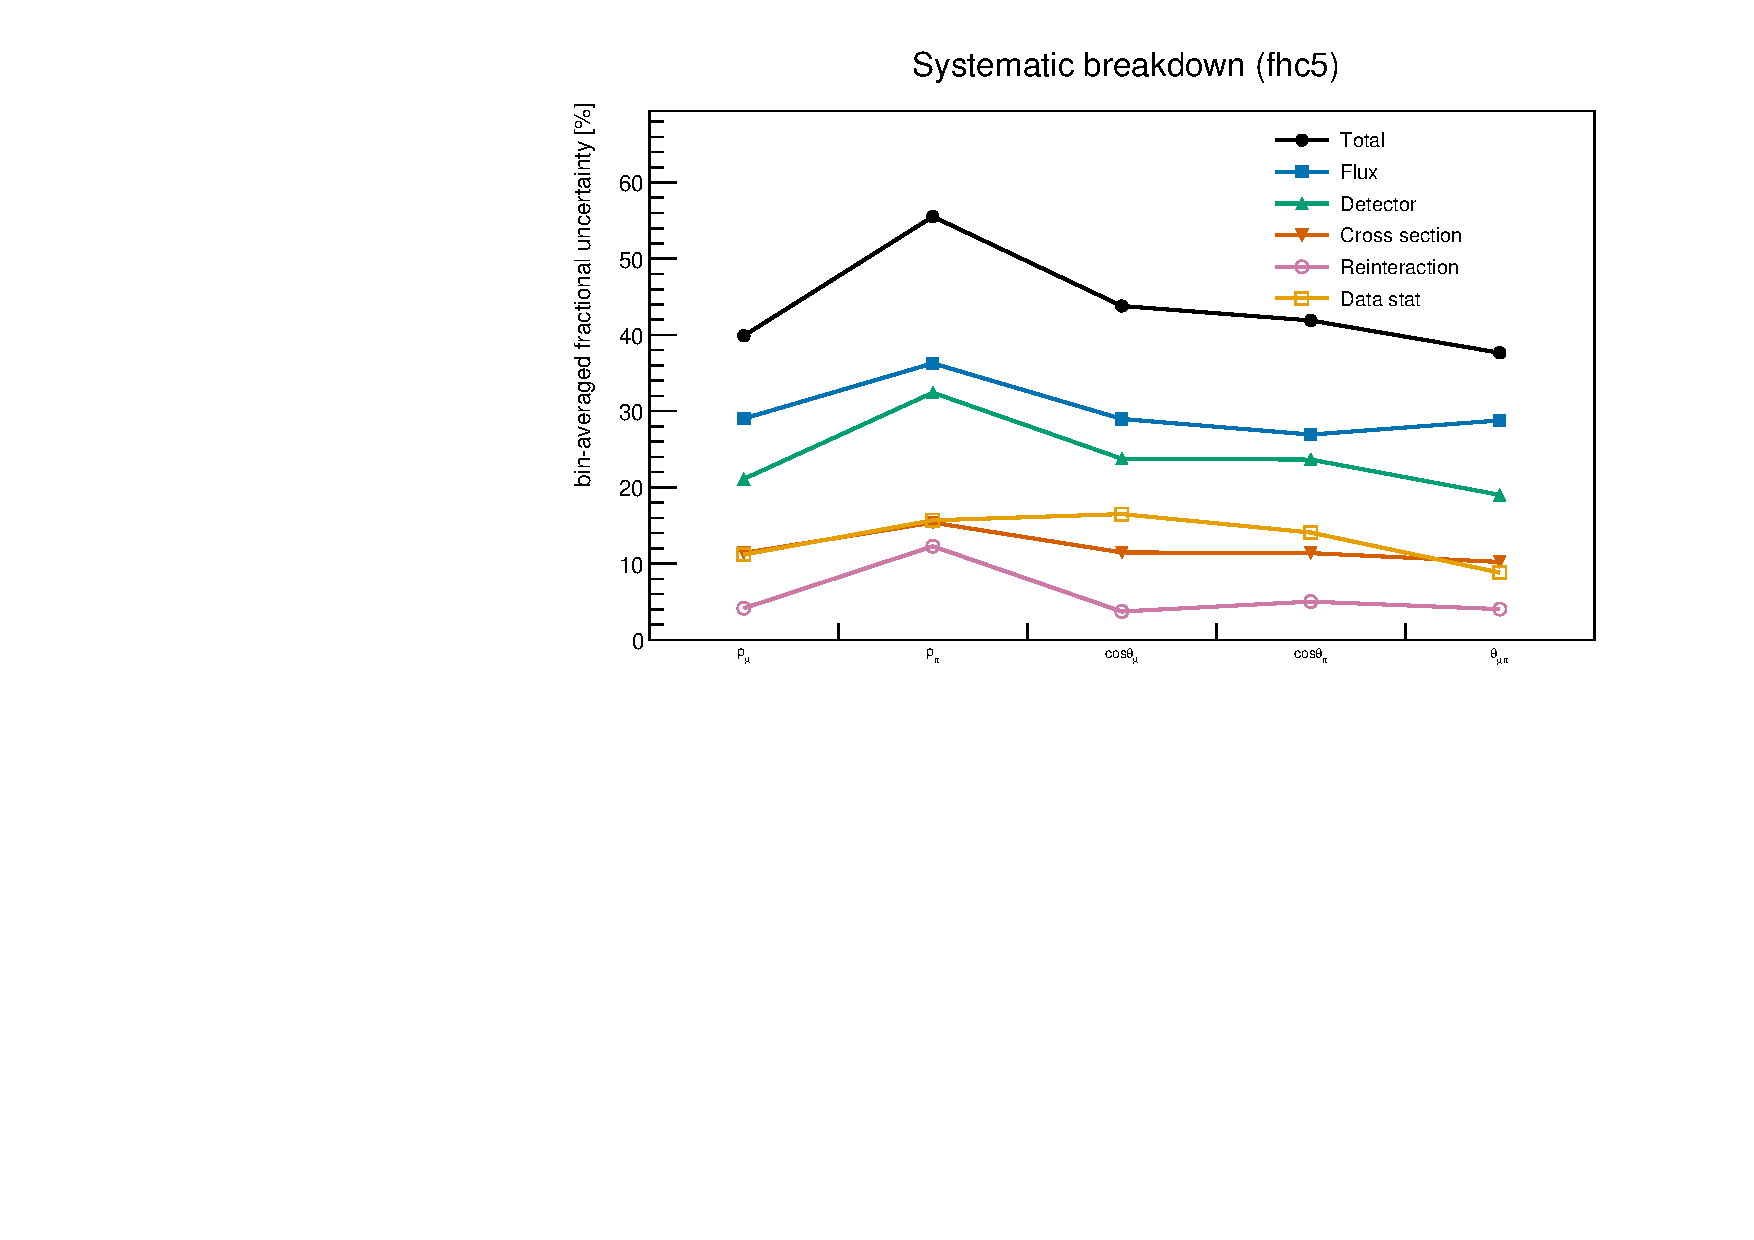
\includegraphics[width=0.49\textwidth]{fw_systbreak_fhc}\hfill
  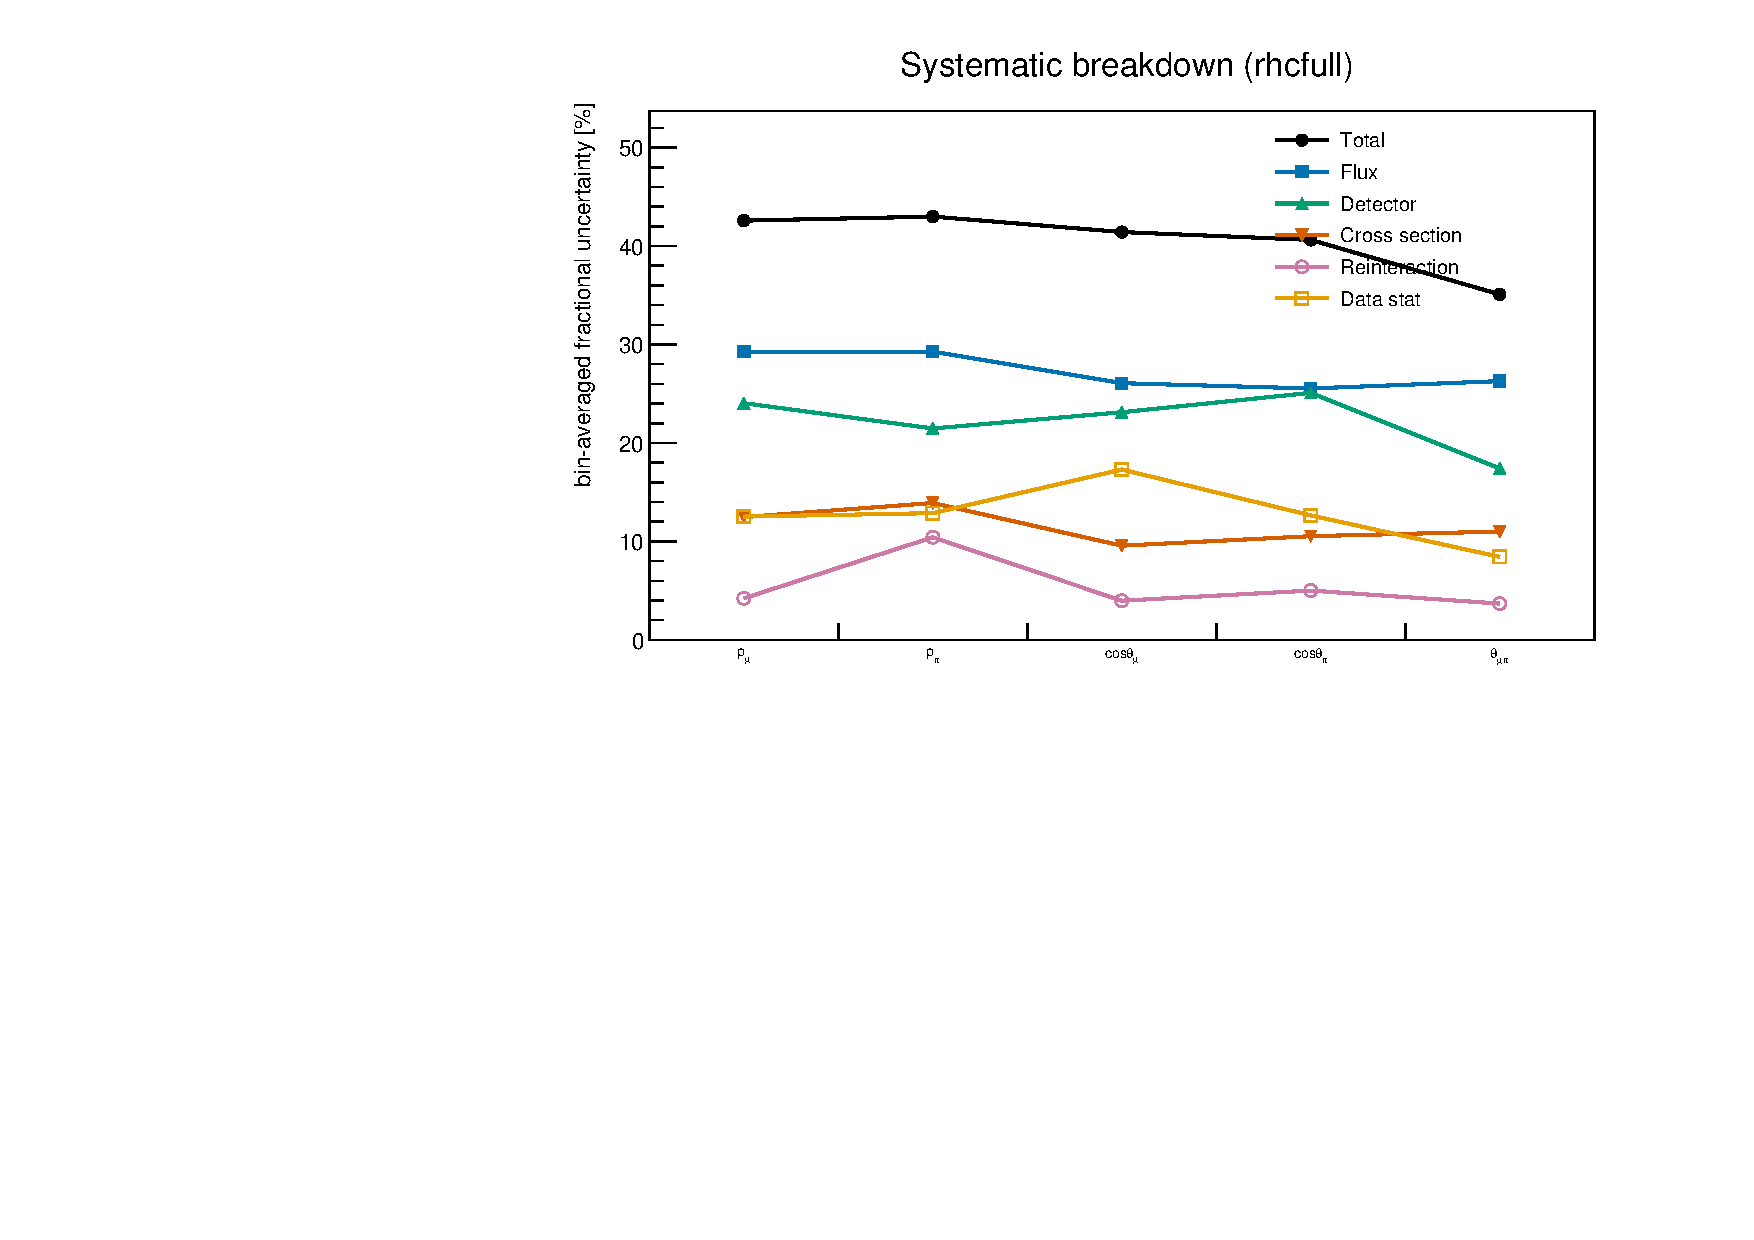
\includegraphics[width=0.49\textwidth]{fw_systbreak_rhc}\\[1mm]
  \scriptsize\raggedright
  \begin{itemize}\setlength\itemsep{1pt}
    \item Flux and detector dominate; data statistics is smaller in every observable.
    \item Combined configuration: the 600 PPFX universes are index-matched in all 14 overlays, so the
      FHC--RHC flux correlation is built in; detector variations pooled once per mode.
    \item Per-observable tables for all three configurations in backup.
  \end{itemize}
  \end{columns}
\end{frame}

\begin{frame}{The flux term: normalisation times $(1+B/S)$}
  \begin{columns}[T]
  \column{.55\textwidth}
  \small
  \begin{itemize}\setlength\itemsep{3pt}
    \item Flux normalisation uncertainty $\approx17\%$; flux term of the one-bin total $28$--$30\%$.
    \item A flux universe moves signal and neutrino background together; $B$ and $\Phi$ move together in
      $(N-B)/(\varepsilon\Phi N_\mathrm{Ar})$:
      \[\frac{\delta\sigma}{\sigma}=\frac{\delta\Phi}{\Phi}\Big(1+\frac{B}{S}\Big)\]
    \item FHC: $17.7\%\times(1+560/833)=29.6\%$ vs.\ $29.9\%$ extracted.
    \item RHC: $15\%\times(1+720/1015)=25.6\%$ vs.\ $27.7\%$.
    \item Not an unfolding effect: the one-bin total has no regularisation and carries the same factor.
    \item Reduced only by higher purity or a control-region background constraint.
  \end{itemize}
  \column{.43\textwidth}
  \small
  \textbf{Outside the official covariance}
  \begin{itemize}\scriptsize\setlength\itemsep{2pt}
    \item Beamline-geometry flux (12 unisims): $1.6$--$3.3\%$, adds $\le0.2\%$ to the flux row.
    \item EXT trigger ratios and the Run-1-for-Run-2 beam-off stand-in: a $20\%$ uncertainty would add
      $0.3\%$.
  \end{itemize}
  \vspace{2mm}
  \textbf{Muon momentum scale}
  \begin{itemize}\scriptsize\setlength\itemsep{2pt}
    \item MCS measures $63\%$ of muons, not varied by the detector samples.
    \item Pseudo-data rethrown with MCS momenta $\times(1\pm0.05)$, unfolded with the nominal response;
      half-difference, fully correlated, in the official covariance.
    \item FHC $p_\mu$: $5$--$8\%$ ($\le0.19\sigma$) in the five lower bins, $17\%$ ($0.56\sigma$) in the open top bin.
    \item Zero for observables that do not use $p_\mu$. The $\pm5\%$ size is assumed.
  \end{itemize}
  \end{columns}
\end{frame}

% =====================================================================
\section{Validation}
\begin{frame}{Validation: from the implementation to the model}
  \scriptsize\centering\setlength{\tabcolsep}{3pt}
  \begin{tabular}{@{}p{2.6cm}p{4.3cm}p{6.8cm}@{}}
    \toprule
    Step & Question & Result \\\midrule
    Identity closure & $UR=A_C$ exactly? & All 59 extractions; worst $6.1\times10^{-5}$ relative (FP rounding) \\
    Nominal closure & Truth of CV pseudo-data returned? & Inclusive $\chi^2\le2.39/8$, integral ratios $0.946$--$1.047$ (mean $0.996$); proton-tagged $\chi^2\le6.01/4$ \\
    Ensembles & Statistical uncertainties sized correctly? & 7 inclusive + 10 proton-tagged, 100 members each: pull widths $0.95$--$1.07$ / $0.94$--$1.08$; $68\%$ coverage $63$--$73\%$ \\
    Reweighted models & Follows a model reweighting can reach? & GENIE multisim u545 and $\Delta\to N\pi$ angular: largest bias $1.18\sigma$ (one sparse FHC $\cos\theta_\mu$ bin); RHC $\le0.83\sigma$ \\
    Independent generator & Follows a model reweighting cannot reach? & Not made: the NuWro overlay has 1.76$\times$ the GENIE rate vs.\ 1.6 expected, provenance untraced \\
    Control regions & Background model supported by data? & Pseudo-data only; frozen procedure for beam-on \\
    \bottomrule
  \end{tabular}
  \vspace{3mm}
  \begin{columns}[T]
  \column{.5\textwidth}\scriptsize
  \textbf{Closure $\chi^2$ with the full covariance} clusters near $p=1$: systematic terms are common to
  pseudo-data and reference. It checks the implementation; ensembles test the sizing.
  \column{.48\textwidth}\scriptsize
  \textbf{Ensemble means} sit $0.4$--$1.1\%$ below the reference (pull means $-0.05$ to $-0.11$, RHC total $-0.21$),
  including the unregularised totals; not corrected.
  \end{columns}
\end{frame}

\begin{frame}{Ensembles and reweighted-model pseudo-data}
  \begin{columns}[T]
  \column{.46\textwidth}
  \scriptsize\centering\setlength{\tabcolsep}{2.5pt}
  \textbf{Ensembles} (statistical covariance)\\[1mm]
  \begin{tabular}{lccc}
    \toprule
    Extraction & mean & width & 68/95\% \\\midrule
    $p_\mu$, FHC & $-0.11$ & 1.07 & 64/94 \\
    $\cos\theta_\mu$, FHC & $-0.06$ & 0.97 & 72/95 \\
    $\cos\theta_\mu$, RHC & $-0.05$ & 1.05 & 63/94 \\
    $p_\pi$, comb. & $-0.11$ & 0.95 & 73/96 \\
    total, FHC & $-0.10$ & 0.97 & 67/95 \\
    total, RHC & $-0.21$ & 0.99 & 64/94 \\
    $\cos\theta_\pi\times\cos\theta_\mu$, comb. & & 1.03 & 67/94 \\
    \bottomrule
  \end{tabular}\\[1mm]
  \raggedright
  Each member rethrown run by run, universes rebuilt; pull against CV truth smeared by the member's own
  $A_C$. Chosen to span conditioning ($\cos\theta_\mu$ RHC row sum $0.26$) and the unregularised totals.
  \column{.52\textwidth}
  \scriptsize\centering\setlength{\tabcolsep}{2.5pt}
  \textbf{Reweighted-model pseudo-data}, nominal response\\[1mm]
  \begin{tabular}{llcccc}
    \toprule
    & & \multicolumn{2}{c}{FHC} & \multicolumn{2}{c}{RHC} \\
    Obs. & Model & ratio & bias & ratio & bias \\\midrule
    $p_\mu$ & u545 & 0.920 & $-0.47\sigma$ & 0.783 & $-0.83\sigma$ \\
     & $\Delta$ ang. & 0.992 & $+0.83\sigma$ & 1.027 & $+0.56\sigma$ \\
    $\cos\theta_\mu$ & u545 & 0.942 & $-0.87\sigma$ & 1.059 & $+0.78\sigma$ \\
     & $\Delta$ ang. & 0.816 & $\mathbf{-1.18\sigma}$ & 1.045 & $-0.47\sigma$ \\
    $\cos\theta_\pi$ & u545 & 0.980 & $+0.40\sigma$ & 0.852 & $-0.64\sigma$ \\
     & $\Delta$ ang. & 0.944 & $-0.59\sigma$ & 0.987 & $+0.20\sigma$ \\
    $p_\pi$ & u545 & 0.750 & $-0.70\sigma$ & 0.852 & $-0.36\sigma$ \\
     & $\Delta$ ang. & 1.084 & $+0.34\sigma$ & 1.158 & $+0.55\sigma$ \\
    \bottomrule
  \end{tabular}\\[1mm]
  \raggedright
  u545 changes shapes by up to $29\%$ at $4\%$ rate change. Bins that do not follow the alternative truth
  are sparse ones (near-threshold $p_\pi$, open top $p_\mu$, $\cos\theta_\mu$ bins 1 and 3), with
  uncertainties of $29$--$114\%$. The test should be repeated if the uncertainties shrink substantially.
  \end{columns}
\end{frame}

% =====================================================================
\section{Results}
\begin{frame}{Differential cross sections, FHC}
  \begin{columns}[T]
  \column{.62\textwidth}
  \centering
  \blindfig[\textwidth]{dsigma_FHC5}
  \column{.37\textwidth}
  \scriptsize\setlength{\tabcolsep}{2pt}
  \begin{tabular}{lcccc}
    \toprule
    & $\sigma_\mathrm{int}$ & Flux & Det. & Closure \\\midrule
    $p_\mu$ & 0.814 & $30.0\%$ & $21.2\%$ & $0.82/6$ \\
    $p_\pi$ & 0.830 & $38.5\%$ & $34.2\%$ & $1.01/3$ \\
    $\cos\theta_\mu$ & 0.713 & $26.6\%$ & $25.4\%$ & $2.39/8$ \\
    $\cos\theta_\pi$ & 0.668 & $27.1\%$ & $23.2\%$ & $1.21/5$ \\
    $\theta_{\mu\pi}$ & 0.796 & $28.8\%$ & $19.9\%$ & $0.39/5$ \\
    \bottomrule
  \end{tabular}\\[2mm]
  \begin{itemize}\setlength\itemsep{1pt}
    \item Points: unfolded pseudo-data, total uncertainty. All curves $A_C$-smeared.
    \item $\sigma_\mathrm{int}$ in $10^{-38}$\,cm$^2$/Ar; differs between observables through $A_C$.
    \item Open top bins hatched: height = integral / plotted width.
  \end{itemize}
  \end{columns}
\end{frame}

\begin{frame}{Differential cross sections, RHC and combined}
  \begin{columns}[T]
  \column{.5\textwidth}
  \centering {\small RHC}\\
  \blindfig[0.84\textwidth]{dsigma_RHCFULL}\\[0.5mm]
  \scriptsize\setlength{\tabcolsep}{2pt}
  \begin{tabular}{lccccc}
    \toprule
    & $p_\mu$ & $p_\pi$ & $\cos\theta_\mu$ & $\cos\theta_\pi$ & $\theta_{\mu\pi}$ \\\midrule
    $\sigma_\mathrm{int}$ & 0.644 & 0.727 & 0.694 & 0.615 & 0.831 \\
    Syst.\ total & $42.0\%$ & $41.1\%$ & $36.9\%$ & $38.5\%$ & $32.6\%$ \\
    Closure $\chi^2$ & 0.44/6 & 0.01/3 & 0.98/8 & 0.49/5 & 0.18/5 \\
    \bottomrule
  \end{tabular}
  \column{.5\textwidth}
  \centering {\small Combined}\\
  \blindfig[0.84\textwidth]{dsigma_COMB}\\[0.5mm]
  \scriptsize\setlength{\tabcolsep}{2pt}
  \begin{tabular}{lccccc}
    \toprule
    & $p_\mu$ & $p_\pi$ & $\cos\theta_\mu$ & $\cos\theta_\pi$ & $\theta_{\mu\pi}$ \\\midrule
    $\sigma_\mathrm{int}$ & 0.742 & 0.762 & 0.744 & 0.649 & 0.860 \\
    Syst.\ total & $40.1\%$ & $45.9\%$ & $33.1\%$ & $37.5\%$ & $33.6\%$ \\
    Closure $\chi^2$ & 0.08/6 & 0.21/3 & 1.29/8 & 0.58/5 & 0.21/5 \\
    \bottomrule
  \end{tabular}
  \end{columns}
  {\tiny Generator predictions averaged over the flux of each configuration; combined: fluence-weighted average ($0.425$ FHC, $0.575$ RHC).}
\end{frame}

\begin{frame}{Pion momentum in three regions and model comparisons}
  \begin{columns}[T]
  \column{.47\textwidth}
  \scriptsize\centering\setlength{\tabcolsep}{2.5pt}
  \textbf{$p_\pi$ as bin integrals} ($10^{-38}$\,cm$^2$/Ar)\\[1mm]
  \begin{tabular}{lccc}
    \toprule
    Region & FHC & RHC & Comb. \\\midrule
    $0.175$--$0.205$ & $0.048\pm0.036$ & $0.064\pm0.029$ & $0.059\pm0.032$ \\
    $0.205$--$0.26$ & $0.086\pm0.061$ & $0.110\pm0.049$ & $0.102\pm0.053$ \\
    $>0.26$ & $0.695\pm0.236$ & $0.553\pm0.222$ & $0.601\pm0.216$ \\
    \bottomrule
  \end{tabular}\\[2mm]
  \raggedright
  \begin{itemize}\setlength\itemsep{1pt}
    \item Range estimator saturates near $0.34\GeVc$: pions interact before stopping.
    \item Diagonals $91/51/52\%$; the two near-threshold regions are measured as a pair
      ($A_C$ mixes them strongly, trace $1.57$).
    \item Upper region is open: compare bin integrals after $A_C$, not densities.
  \end{itemize}
  \column{.51\textwidth}
  \scriptsize\centering\setlength{\tabcolsep}{2pt}
  \textbf{$\chi^2$/ndf against $A_C$-smeared predictions}, full covariance\\[1mm]
  \begin{tabular}{llcccccc}
    \toprule
    & & truth & tune & GENIE & GiBUU & NEUT & NuWro \\\midrule
    FHC & $p_\mu$ & 0.82 & 1.29 & 2.24 & 1.27 & 2.27 & 1.35 \\
     & $p_\pi$ & 1.01 & 1.20 & 1.56 & 4.13 & 1.83 & 2.26 \\
     & $\cos\theta_\mu$ & 2.39 & 1.75 & 2.37 & 2.57 & 3.93 & 4.88 \\
     & $\cos\theta_\pi$ & 1.21 & 1.21 & 1.92 & 2.56 & 2.26 & 3.09 \\
     & $\theta_{\mu\pi}$ & 0.39 & 0.47 & 0.82 & 0.67 & 2.71 & 3.16 \\\midrule
    RHC & $\cos\theta_\mu$ & 0.98 & 1.27 & 1.84 & 0.71 & 6.36 & 10.39 \\\midrule
    comb & $\cos\theta_\mu$ & 1.29 & 1.17 & 2.17 & 1.30 & 5.24 & 9.52 \\
    \bottomrule
  \end{tabular}\\[1mm]
  \raggedright
  ndf = 6, 3, 8, 5, 5. Full table in backup. With pseudo-data from the tune, these test the procedure;
  the spread shows the model differences the measurement is expected to resolve.
  $A_C$ is applied once; applying it twice created a spurious NEUT/NuWro separation (fixed).
  \end{columns}
\end{frame}

\begin{frame}{Total cross section: one-bin extraction}
  \begin{columns}[T]
  \column{.56\textwidth}
  \small
  \[\sigma=\frac{N_\mathrm{sel}-N_\mathrm{bkg}}{\varepsilon\,\Phi\,N_\mathrm{Ar}},\qquad A_C\equiv1\]
  \begin{itemize}\scriptsize\setlength\itemsep{2pt}
    \item One true and one reco bin over $\cos\theta_\mu\in[-1,1]$; Wiener filter off; every term
      evaluated universe by universe.
    \item Closed-form evaluation reproduces the CV one-bin extraction to four digits ($1.0315$, $0.9285$, $0.9723$).
    \item Flux $28$--$30\%$, detector $20$--$22\%$, data statistics $3$--$5\%$.
    \item RHC/FHC: tune $0.900$, extracted $0.901$.
    \item The one-bin total lies above the $A_C$-suppressed $\sigma_\mathrm{int}$ and agrees with D'Agostini.
  \end{itemize}
  \column{.42\textwidth}
  \scriptsize\centering\setlength{\tabcolsep}{2pt}
  \textbf{Generators vs.\ one-bin total} ($10^{-38}$\,cm$^2$/Ar)\\[1mm]
  \begin{tabular}{lccc}
    \toprule
    & FHC & RHC & Comb. \\\midrule
    Measured & $1.03\pm0.40$ & $0.93\pm0.35$ & $0.98\pm0.37$ \\
    GENIE & 0.82 & 0.67 & 0.73 \\
    GiBUU & 1.13 & 0.94 & 1.02 \\
    NEUT & 1.32 & 1.10 & 1.20 \\
    NuWro & 1.25 & 1.04 & 1.13 \\
    \bottomrule
  \end{tabular}\\[1mm]
  All within $0.8\sigma$; generator spread a factor $1.6$.
  \end{columns}
  \vspace{2mm}
  \centering\scriptsize\setlength{\tabcolsep}{3pt}
  \begin{tabular}{lrrcccccccc}
    \toprule
    Config & $N_\mathrm{sel}$ & $N_\mathrm{bkg}$ & $\varepsilon$ & $\sigma$ & stat & syst & total & truth & $\sigma$/truth & $\chi^2/1$ \\\midrule
    FHC & 1\,423 & 590 & $17.5\%$ & $1.034\pm0.396$ & $4.5\%$ & $38.0\%$ & $38.3\%$ & 1.044 & 0.991 & 0.001 \\
    RHC & 1\,768 & 752 & $17.6\%$ & $0.932\pm0.350$ & $4.1\%$ & $37.4\%$ & $37.6\%$ & 0.941 & 0.990 & 0.001 \\
    Combined & 3\,191 & 1\,342 & $17.5\%$ & $0.975\pm0.366$ & $3.0\%$ & $37.5\%$ & $37.6\%$ & 0.985 & 0.990 & 0.001 \\
    \bottomrule
  \end{tabular}
\end{frame}

\begin{frame}{Two-dimensional $d^2\sigma/d\cos\theta_\pi\,d\cos\theta_\mu$ (combined, secondary)}
  \centering
  \blindfig[0.8\textwidth]{bkgfit/xsec2d_costhpi_costhmu_COMB_slices}
  \begin{columns}[T]
  \column{.5\textwidth}
  \begin{itemize}\scriptsize\setlength\itemsep{1pt}
    \item $\cos\theta_\pi$: $-1$, $0.35$, $1$ inside $\cos\theta_\mu$: $-1$, $0.65$, $0.85$, $1$ (6 bins).
    \item Combining modes raises the $A_C$ conditioning from $0.245$ (FHC), $0.315$ (RHC) to $0.564$; single-mode
      extractions not reported.
    \item Closure $\chi^2=0.88/6$, cell ratios $0.91$--$1.26$; per-bin uncertainty $33$--$64\%$.
  \end{itemize}
  \column{.48\textwidth}
  \begin{itemize}\scriptsize\setlength\itemsep{1pt}
    \item Ensemble: pull width $1.03$, coverage $67/94\%$.
    \item Sparsest cell $11\%$ low on average ($0.58$ stat.\ s.d., $0.17$ of its total), not corrected.
    \item Reweighted models: every cell within $0.61\sigma$.
  \end{itemize}
  \end{columns}
\end{frame}

% =====================================================================
\section{Proton-tagged}
\begin{frame}{Proton-tagged subsample: selection and observables}
  \begin{columns}[T]
  \column{.5\textwidth}
  \small
  \textbf{Signal}: inclusive signal with $\ge1$ true proton above $0.3\GeVc$; leading proton for truth observables.\\[1mm]
  \textbf{Cut 11}: most proton-like remaining track (LLR $<0.05$), contained, $p_p\ge0.3\GeVc$ (range KE).\\[2mm]
  \scriptsize\setlength{\tabcolsep}{3pt}
  \begin{tabular}{lccc}
    \toprule
    & FHC & RHC & Comb. \\\midrule
    Efficiency & $11.5\%$ & $11.4\%$ & $11.5\%$ \\
    Purity & $52\%$ & $50\%$ & $51\%$ \\
    \bottomrule
  \end{tabular}\\[1mm]
  \begin{itemize}\setlength\itemsep{1pt}
    \item Rejects $67\%$ of the neutrino background for $32\%$ signal loss; EXT down $\times3.3$--$3.6$.
    \item Candidate is the leading true proton in $81.7\%$, some proton in $87.4\%$, not a proton in $12.6\%$.
    \item Wrong candidates dominate the $\theta_p$ tails ($74\%$ of residuals beyond $0.3$\,rad).
  \end{itemize}
  \column{.48\textwidth}
  \scriptsize
  \textbf{Observables} (about the $\nu$ direction)
  \begin{itemize}\setlength\itemsep{1pt}
    \item $p_p$ (3), $\theta_p$ (4), $\theta_{\pi p}$ (4)
    \item $W_\mathrm{had}$ (2 regions, split $1.18$\,GeV/$c^2$)
    \item TKI of $\mu$ vs.\ $(\pi+p)$: $\delta p_T$ (2), $\delta\alpha_T$ (2), $\delta\phi_T$ (3), $p_n$ (2)
    \item $p_\mu$, $p_\pi$ (2), $\cos\theta_\mu$, $\cos\theta_\pi$ (4), $\theta_{\mu\pi}$ again on this phase space
  \end{itemize}
  Binnings: $0.50$ criterion, $\ge50$ selected FHC signal per bin.\\[2mm]
  \textbf{Status}
  \begin{itemize}\setlength\itemsep{1pt}
    \item One-bin total, $d\sigma/d\theta_p$, $d\sigma/d\theta_{\pi p}$ (3 configs), $d^2\sigma/d\theta_p\,d\delta p_T$ (combined).
    \item $W_\mathrm{had}$, TKI, $p_p$ and the $\mu$/$\pi$ observables are released as validation-only products.
    \item No differential $W_{\pi p}$ result.
  \end{itemize}
  Detector term $9.9$--$74.5\%$ (median $30.9\%$).
  \end{columns}
\end{frame}

\begin{frame}{Proton-tagged results}
  \begin{columns}[T]
  \column{.56\textwidth}
  \centering
  \blindfig[\textwidth]{newobs_xsec}\\
  {\scriptsize $\theta_p$ (top) and $\theta_{\pi p}$ (bottom), FHC, RHC, combined.}
  \column{.42\textwidth}
  \scriptsize\centering\setlength{\tabcolsep}{2pt}
  \textbf{One-bin total} ($10^{-38}$\,cm$^2$/Ar)\\[1mm]
  \begin{tabular}{lcccc}
    \toprule
    & $\sigma$ & total & truth & $\sigma$/truth \\\midrule
    FHC & $0.608\pm0.256$ & $42.0\%$ & 0.639 & 0.952 \\
    RHC & $0.531\pm0.251$ & $47.2\%$ & 0.532 & 0.998 \\
    Comb. & $0.564\pm0.239$ & $42.5\%$ & 0.578 & 0.976 \\
    \bottomrule
  \end{tabular}\\[1mm]
  \raggedright
  FHC generators: GENIE $0.50$, NuWro $0.65$, GiBUU $0.74$, NEUT $0.78$; tune $0.63$.
  RHC/FHC $0.873$ (tune $0.878$).
  \begin{itemize}\setlength\itemsep{1pt}
    \item $\theta_{\pi p}$: trace $2.1$--$2.2$, three components with S/N $>1$ (FHC, RHC); last bin $94$--$141\%$.
    \item $\theta_p$: trace $2.1$--$2.3$; largest per-bin $41\%$ (FHC), $84\%$ (RHC).
    \item Ensembles: widths $0.94$--$1.03$; reweighted models $\le0.79\sigma$.
    \item Generators differ mainly in normalisation.
  \end{itemize}
  \end{columns}
\end{frame}

\begin{frame}{Proton-tagged: TKI, $W_\mathrm{had}$ and model sensitivity}
  \begin{columns}[T]
  \column{.58\textwidth}
  \centering
  \blindfig[0.86\textwidth]{dsigma_ccpi1p_noW_FHC5_b}\\[0.5mm]
  \blindfig[0.86\textwidth]{dsigma_ccpi1p_noW_FHC5_a}\\
  {\scriptsize FHC: $\delta p_T$, $\delta\alpha_T$, $\delta\phi_T$ (top); $W_\mathrm{had}$, $p_p$, $p_n$ (bottom).}
  \column{.4\textwidth}
  \scriptsize
  \begin{itemize}\setlength\itemsep{2pt}
    \item Closure: $\chi^2\le6.01/4$ (RHC $\cos\theta_\pi$), integral ratios $0.93$--$1.18$.
    \item All generators compatible with the pseudo-data; largest $\chi^2$ $4.1/2$ (GENIE, comb.\ $p_n$).
    \item Under GENIE u545 the low $\delta p_T$ and $p_n$ bins return $35\%$ low ($-1.14\sigma$, $-1.16\sigma$)
      while their truth moves $1\%$: the change enters through sample composition and proton-tag efficiency.
    \item $W_\mathrm{had}$ and $p_n$ use a residual-mass prescription derived for QE kinematics, not
      validated for pion production.
    \item MCS scale term recomputed for $W_\mathrm{had}$, $\delta p_T$, $\delta\alpha_T$, $p_n$: $\le0.37\sigma$.
  \end{itemize}
  \vspace{1mm}
  \textbf{Why no $W_{\pi p}$}: six bins have diagonals down to $2\%$; the best two-bin split passes $0.50$ by
  $0.003$ with a second filter factor $0.27$--$0.29$ (normalisation only).
  \end{columns}
\end{frame}

% =====================================================================
\section{Limitations and summary}
\begin{frame}{Limitations}
  \begin{columns}[T]
  \column{.5\textwidth}
  \small
  \begin{itemize}\setlength\itemsep{4pt}
    \item \textbf{Blind signal region}: results demonstrate the extraction and its uncertainties, not the
      cross section. At $57$--$59\%$ purity the background model enters strongly; closure cannot test it.
    \item \textbf{Pion momentum}: saturation near $0.34\GeVc$; golden pion, MCS, calorimetry, regression,
      daughter recovery and the proton tag all tried. A truth-level golden selection does no better than
      the classifier, so the limit is physical.
    \item \textbf{Model dependence}: reweighting bounds the bias at $1.18\sigma$; no independent-generator
      closure. Efficiency model dependence matters most for the one-bin total and the open $p_\pi>0.26$ region.
  \end{itemize}
  \column{.48\textwidth}
  \small
  \begin{itemize}\setlength\itemsep{4pt}
    \item \textbf{Muon momentum scale}: $\pm5\%$ assumed, not yet compared with MCS vs.\ range on contained muons in data.
    \item \textbf{Proton-tagged}: no control region constrains the $12.6\%$ pion$\to$proton mis-assignment
      (an inverted proton-PID region is not defined); no covariance term for the TKI model sensitivity.
    \item \textbf{Background control regions}: studied with pseudo-data; beam-on comparison follows the frozen procedure.
  \end{itemize}
  \end{columns}
\end{frame}

\begin{frame}{Summary}
  \footnotesize
  \begin{itemize}\setlength\itemsep{3pt}
    \item $\nu_\mu+\bar\nu_\mu$ CC$\pi^\pm$ on argon with the full NuMI exposure: FHC $7.766$, RHC $11.082$,
      combined $18.848\times10^{20}$\,POT. Blind; all results from CV pseudo-data.
    \item Selection: $17.5\%$ efficiency at $57$--$59\%$ purity; angles about the per-event $\nu$ direction,
      $28.6^\circ$ from the detector axis.
    \item Primary results: $d\sigma/dp_\mu$, $d\sigma/d\cos\theta_\mu$, $d\sigma/d\cos\theta_\pi$,
      $d\sigma/d\theta_{\mu\pi}$, $p_\pi$ in three regions, and the one-bin total, in three configurations.
      Secondary: combined $\cos\theta_\pi\times\cos\theta_\mu$.
    \item Total: $38\%$ uncertainty (flux $28$--$30\%$ = $17\%\times(1+B/S)$, detector $20$--$22\%$).
      Differential: $33$--$46\%$ bin-averaged without data statistics.
    \item Every result released with $A_C$ and covariance by source; binnings meet the $0.50$ migration criterion.
    \item Validation: closure mean ratio $0.996$; ensemble pull widths $0.95$--$1.07$; reweighted-model
      bias $\le1.18\sigma$; $UR=A_C$ to $6.1\times10^{-5}$; independent rebuild reproduces all 51 extractions to $10^{-9}$.
    \item Proton-tagged: one-bin total, $\theta_p$, $\theta_{\pi p}$ and combined $\theta_p\times\delta p_T$;
      $11.5\%$ efficiency, $50$--$52\%$ purity.
    \item Outstanding before unblinding: beam-on control-region comparison, independent-generator closure.
  \end{itemize}
  \label{mainend}
\end{frame}

% =====================================================================
% BACKUP: technical supplement
% =====================================================================
\backuptrue
\appendix
\section{Backup}
{\setbeamertemplate{footline}{}
\begin{frame}[plain]
  \centering\vfill
  {\Huge\color{ubred}Backup}\\[4mm]
  {\large Technical supplement v1.6}\\[3mm]
  \small Final configuration $\cdot$ evidence for the choices $\cdot$ rejected alternatives
  \vfill
\end{frame}}

\begin{frame}{Backup: final binnings and the binning rule}
  \begin{columns}[T]
  \column{.5\textwidth}
  \scriptsize
  \textbf{Rule} (binning review, 2026-09-26)
  \begin{enumerate}\setlength\itemsep{0pt}
    \item Maximin partition for every bin count up to 12 (largest worst diagonal over FHC and RHC; dynamic programming, \texttt{maximin\_binning.py}).
    \item Event floor: $\ge70$ selected FHC signal (inclusive), $\ge50$ (proton-tagged).
    \item Every diagonal $\ge0.50$ in FHC and RHC on the analysis sample.
    \item Extract candidates in full, three configurations.
    \item Wiener filter factors; trace of $A_C$.
    \item Fewest bins reaching $90\%$ of the largest trace (FHC/RHC average); ties to larger worst diagonal.
    \item Check closure and per-bin uncertainties.
    \item Freeze.
  \end{enumerate}
  \textbf{Exceptions}: $\cos\theta_\pi$ and $\theta_{\mu\pi}$ keep 5 bins; $\delta\alpha_T$ keeps $120^\circ$;
  proton-tagged $p_\pi$ keeps 2 regions. $153$ extractions in the review.
  \column{.48\textwidth}
  \scriptsize\centering\setlength{\tabcolsep}{2pt}
  \textbf{Proton-tagged edges}\\[1mm]
  \begin{tabular}{lcl}
    \toprule
    Obs. & bins & edges \\\midrule
    $p_\pi$ & 2 & 0.175, 0.205, open \\
    $\cos\theta_\pi$ & 4 & $-1$, $-0.1$, 0.35, 0.75, 1 \\
    $W_\mathrm{had}$ & 2 & 0, 1.18, open \\
    $\delta p_T$ & 2 & 0, 0.3, open \\
    $\delta\phi_T$ & 3 & 0, 22.5, 75, 180$^\circ$ \\
    $\delta\alpha_T$ & 2 & 0, 120, 180$^\circ$ \\
    $p_n$ & 2 & 0, 0.375, open \\
    $p_p$ & 3 & 0.3, 0.42, 0.6, open \\
    $\theta_p$ & 4 & 0, 0.44, 0.785, 1.162, $\pi$ \\
    $\theta_{\pi p}$ & 4 & 0, 0.911, 1.414, 1.916, $\pi$ \\
    \bottomrule
  \end{tabular}\\[1mm]
  \raggedright $p_\mu$, $\cos\theta_\mu$, $\theta_{\mu\pi}$ use the inclusive edges. Open bins are drawn with
  a conventional width; the bin integral is the quantity.
  \end{columns}
\end{frame}

\begin{frame}{Backup: binning review, $0.68$ vs.\ $0.50$}
  \begin{columns}[T]
  \column{.58\textwidth}
  \centering
  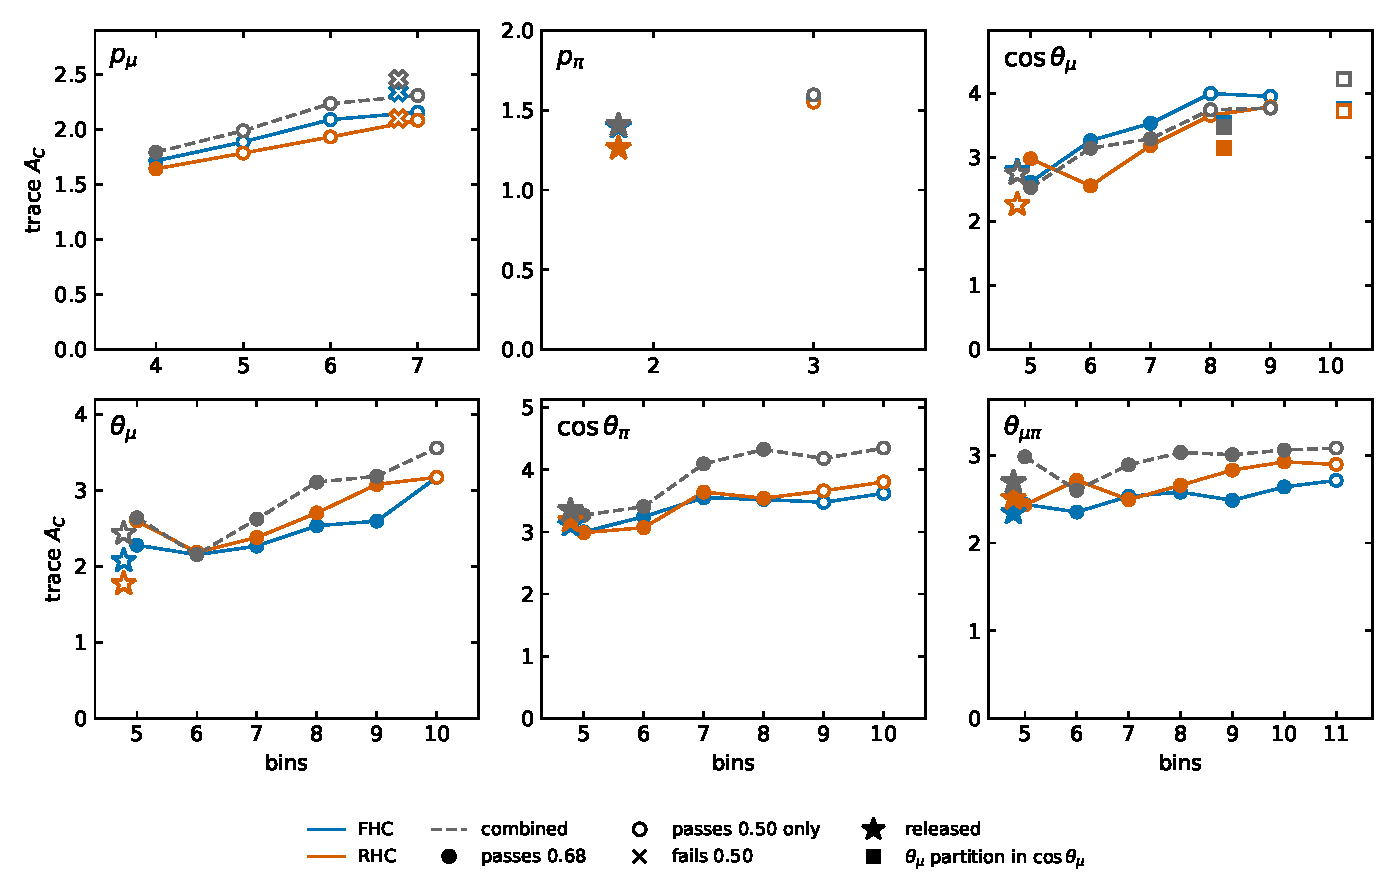
\includegraphics[width=\textwidth]{binreview_dfs_incl}\\
  {\scriptsize Trace of $A_C$ vs.\ number of bins, inclusive. Filled: passes $0.68$; open: $0.50$ only; cross: neither.}
  \column{.4\textwidth}
  \scriptsize
  \begin{itemize}\setlength\itemsep{2pt}
    \item Where the criteria differ, $0.50$ adds $0.2$--$0.6$ degrees of freedom per beam:
      $p_\mu$ 6 vs.\ 4, $p_\pi$ 3 vs.\ 2, $\cos\theta_\mu$ 8 vs.\ 7, $\delta\phi_T$ 3 vs.\ 2, $\theta_{\pi p}$ 4 vs.\ 3.
    \item $0.68$ would drop $p_\mu$ from three well-measured components to two.
    \item Released 7-bin $p_\mu$ failed both (diagonal down to $0.33$); 6-bin $W_\mathrm{had}$ failed both.
    \item $\cos\theta_\pi$ at 7 bins would add $0.45$ d.o.f.; kept at 5.
    \item $\theta_{\mu\pi}$ carries $\approx2.5$ d.o.f.\ however it is binned.
    \item Conditioning $s_\mathrm{min}/s_1$ replaced by the trace: it is set by the weakest component alone.
  \end{itemize}
  \end{columns}
\end{frame}

\begin{frame}{Backup: pion momentum saturation}
  \begin{columns}[T]
  \column{.47\textwidth}
  \centering
  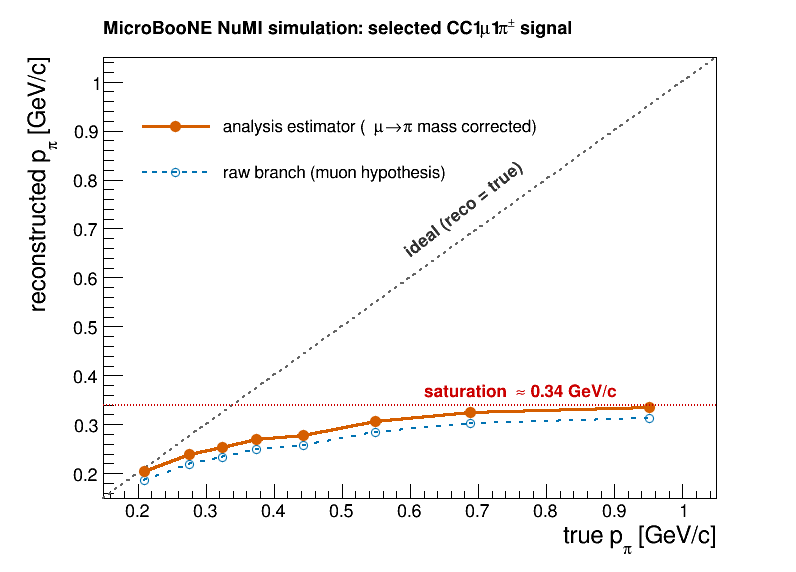
\includegraphics[width=\textwidth]{ppi_saturation}
  \column{.51\textwidth}
  \scriptsize\centering\setlength{\tabcolsep}{2.5pt}
  \begin{tabular}{lrccc}
    \toprule
    true $p_\pi$ & $N$ & $\langle p^\mathrm{true}\rangle$ & $\langle p^\mathrm{corr}\rangle$ & corr./true \\\midrule
    0.175--0.250 & 528 & 0.210 & 0.205 & 0.976 \\
    0.250--0.300 & 270 & 0.276 & 0.238 & 0.863 \\
    0.300--0.350 & 254 & 0.325 & 0.253 & 0.779 \\
    0.350--0.400 & 265 & 0.374 & 0.270 & 0.721 \\
    0.400--0.500 & 403 & 0.443 & 0.279 & 0.629 \\
    0.500--0.600 & 252 & 0.548 & 0.307 & 0.560 \\
    0.600--0.800 & 272 & 0.688 & 0.326 & 0.473 \\
    0.800--1.200 & 164 & 0.951 & 0.336 & 0.353 \\
    \bottomrule
  \end{tabular}\\[1mm]
  \raggedright
  \begin{itemize}\setlength\itemsep{1pt}
    \item $\mu\to\pi$ mass swap fixes the hypothesis bias; nothing fixes the hadronic truncation.
    \item Five-bin diagonals $94/37/23/10/6\%$: every true bin piles into reco bin 1.
    \item Two regions: $91/76\%$ (passes $0.68$); three regions: $91/51/52\%$ (passes $0.50$).
    \item First edge $0.205$: narrowest interval with BNB precedent ($30$\,MeV/$c$); best in every edge scan.
    \item Proton tag does not change the pion response ($88.9/74.2\%$ vs.\ $91.0/75.5\%$).
  \end{itemize}
  \end{columns}
\end{frame}

\begin{frame}{Backup: pion momentum estimators and the golden-pion classifier}
  \begin{columns}[T]
  \column{.5\textwidth}
  \scriptsize\centering\setlength{\tabcolsep}{2.5pt}
  \textbf{Golden-pion BDT}, held-out Run 2, track sample\\[1mm]
  \begin{tabular}{lcccccc}
    \toprule
    cut & eff. & golden & b2 & b3 & b4 & b5 \\\midrule
    none & $100\%$ & $43.1\%$ & 23.7 & 13.2 & 6.4 & 5.5 \\
    $>0.00$ & $44.8\%$ & $64.9\%$ & 33.1 & 24.5 & 15.4 & 9.1 \\
    $>+0.15$ & $15.2\%$ & $84.5\%$ & 46.9 & 42.2 & 36.1 & 19.5 \\\midrule
    truth golden & $43.1\%$ & $100\%$ & 36.1 & 24.1 & 14.2 & 8.9 \\
    \bottomrule
  \end{tabular}\\[1mm]
  \raggedright
  ROC $0.758$; reproduces the BNB benchmark ($36\to68\%$ golden). At matched efficiency the classifier
  equals perfect truth selection bin by bin: no better classifier can repair the response. BNB meets $0.68$
  because its resolved bins lie below $0.175\GeVc$.
  \column{.48\textwidth}
  \scriptsize\centering\setlength{\tabcolsep}{3pt}
  \textbf{Estimators without a magnetic field}\\[1mm]
  \begin{tabular}{lccl}
    \toprule
    estimator & reco/true (top) & RMS & \\\midrule
    range & 0.319 & 0.16 & saturates \\
    calorimetric & 0.383 & 0.31 & truncated, noisier \\
    MCS & 1.011 & 2.1 & unusable on short tracks \\
    golden selection & 0.327 & 0.18 & no gain $>0.8$ \\
    \bottomrule
  \end{tabular}\\[2mm]
  \raggedright
  A pion that interacts before stopping destroys the information a non-magnetised detector uses. Regression
  removes the $W_{\pi p}$ bias at the cost of model dependence. Not tried: TKI constraint on $p_T^\pi$ in the
  proton-tagged sample (limited by Fermi motion, $\approx250$\,MeV/$c$).
  \end{columns}
\end{frame}

\begin{frame}{Backup: three-region $p_\pi$ result and its $A_C$}
  \begin{columns}[T]
  \column{.34\textwidth}
  \centering
  \blindfig[\textwidth]{ppi3bin_xsec_FHC}\\
  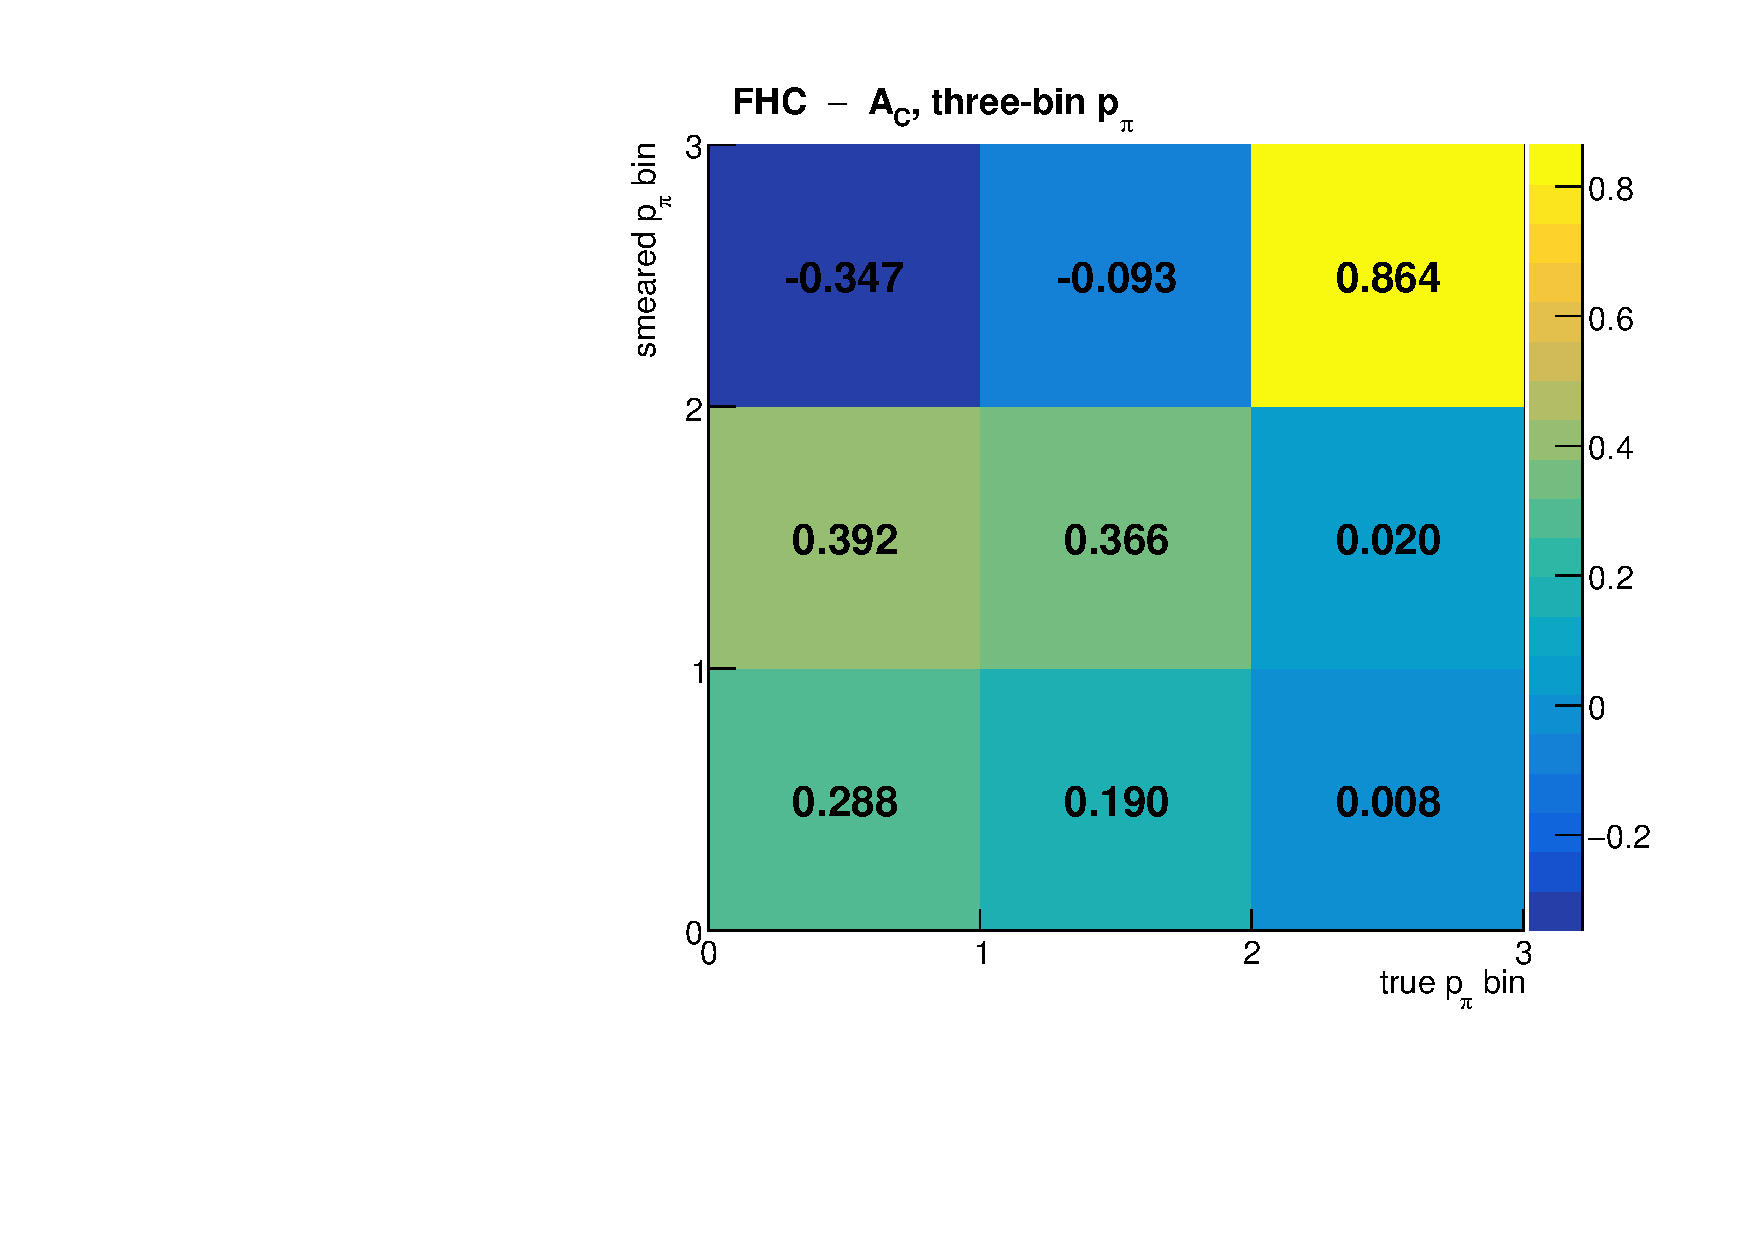
\includegraphics[width=0.8\textwidth]{ppi3bin_AC_FHC}
  \column{.64\textwidth}
  \scriptsize\centering\setlength{\tabcolsep}{2pt}
  $d\sigma/dp_\pi$ [$10^{-38}$\,cm$^2$/(GeV/$c$)/Ar], all curves $A_C$-smeared\\[1mm]
  \begin{tabular}{lccc|ccc|ccc}
    \toprule
    & \multicolumn{3}{c|}{FHC} & \multicolumn{3}{c|}{RHC} & \multicolumn{3}{c}{Comb.} \\
    & b1 & b2 & b3 & b1 & b2 & b3 & b1 & b2 & b3 \\\midrule
    unfolded & 1.62 & 1.57 & 0.94 & 2.14 & 2.00 & 0.75 & 1.97 & 1.85 & 0.81 \\
    unc. & 1.21 & 1.11 & 0.32 & 0.96 & 0.89 & 0.30 & 1.05 & 0.97 & 0.29 \\
    $A_C$ truth & 2.39 & 2.21 & 0.85 & 2.10 & 1.97 & 0.77 & 2.24 & 2.07 & 0.78 \\\midrule
    GENIE & 1.91 & 1.77 & 0.67 & 1.57 & 1.47 & 0.53 & 1.73 & 1.60 & 0.58 \\
    GiBUU & 3.29 & 2.97 & 0.83 & 2.64 & 2.44 & 0.67 & 2.91 & 2.62 & 0.72 \\
    NEUT & 3.09 & 2.83 & 1.08 & 2.56 & 2.39 & 0.88 & 2.77 & 2.53 & 0.94 \\
    NuWro & 3.16 & 2.91 & 0.97 & 2.63 & 2.45 & 0.80 & 2.88 & 2.66 & 0.85 \\\midrule
    $\chi^2$ & \multicolumn{3}{c|}{1.01/3} & \multicolumn{3}{c|}{0.01/3} & \multicolumn{3}{c}{0.21/3} \\
    \bottomrule
  \end{tabular}\\[2mm]
  \raggedright
  FHC $A_C=\left(\begin{smallmatrix}0.40&0.16&0.01\\0.58&0.32&0.02\\-0.22&-0.11&0.85\end{smallmatrix}\right)$:
  the near-threshold regions are mixed and carry one component together (trace $1.57$). Negative entries are
  the regularisation borrowing between regions. The five-bin extraction also closes ($\chi^2\approx2/5$):
  closure cannot expose a response without shape information; the migration criterion can.
  \end{columns}
\end{frame}

\begin{frame}{Backup: hadronic mass $W_{\pi p}$ is not reported}
  \begin{columns}[T]
  \column{.5\textwidth}
  \scriptsize\centering\setlength{\tabcolsep}{3pt}
  \begin{tabular}{lcc}
    \toprule
    & $W_{\pi p}$ & $W_\mathrm{had}$ \\\midrule
    residual RMS [GeV/$c^2$] & 0.142 & 0.283 \\
    half-width ($16$--$84\%$) & 0.101 & 0.177 \\
    bias & $-0.111$ & $-0.032$ \\
    narrowest six-bin bin & 0.040 & 0.100 \\
    \bottomrule
  \end{tabular}\\[2mm]
  \raggedright
  \begin{itemize}\setlength\itemsep{1pt}
    \item Six-bin $W_{\pi p}$ diagonals $88/22/12/12/10/2\%$: bins 2--3$\times$ narrower than the resolution.
    \item $W_{\pi p}$ inherits the $p_\pi$ saturation.
    \item Low generator $\chi^2$ at six bins reflected a binning that cannot resolve the models, not agreement.
  \end{itemize}
  \column{.48\textwidth}
  \scriptsize
  \textbf{Two bins fail on statistics}
  \begin{center}\setlength{\tabcolsep}{3pt}
  \begin{tabular}{lcc}
    \toprule
    two-bin scheme & $A_C$ & $s_2/s_1$ \\\midrule
    $W_{\pi p}$, $N_1=137$ & $\left(\begin{smallmatrix}0.018&-0.410\\0.034&0.892\end{smallmatrix}\right)$ & 0.031 \\
    $p_\pi$ 1p, $N_1=469$ & $\left(\begin{smallmatrix}0.498&-0.089\\0.013&0.854\end{smallmatrix}\right)$ & 0.577 \\
    $p_\pi$ incl., $N_1=1056$ & $\left(\begin{smallmatrix}0.594&-0.382\\0.011&0.891\end{smallmatrix}\right)$ & 0.528 \\
    \bottomrule
  \end{tabular}
  \end{center}
  \begin{itemize}\setlength\itemsep{1pt}
    \item Narrow enough to pass the criterion leaves bin 1 too sparse; wide enough to unfold ($1.19$, 468 events) fails at $56\%$.
    \item No two- or three-bin scheme between $1.12$ and $1.70$ satisfies both.
    \item $W_\mathrm{had}$ in two regions ($0.71/0.72$) is released as validation-only.
  \end{itemize}
  \end{columns}
\end{frame}

\begin{frame}{Backup: bin widths in the regularisation operator}
  \begin{columns}[T]
  \column{.48\textwidth}
  \small
  \begin{itemize}\setlength\itemsep{3pt}
    \item The $(1,-2,1)$ stencil is a second derivative only on a uniform grid. With width ratios up to
      $14{:}1$ its near-null direction is the constant vector.
    \item The Wiener filter then keeps that direction alone: rank-1 $A_C$, normalisation passed, shape lost.
    \item FHC $\theta_\mu$ (pre-review binning): data, truth, tune and all generators share one shape to 4
      decimals; inputs $s_2/s_1=5\times10^{-2}$, outputs $2.8\times10^{-6}$.
    \item Adopted: density differenced on the actual grid, one-sided first derivative at the ends
      (Dirichlet rejected: $\cos\theta_\mu$ peaks at its edge).
  \end{itemize}
  \column{.5\textwidth}
  \scriptsize\centering\setlength{\tabcolsep}{2.5pt}
  $A_C$ conditioning $s_2/s_1$, uniform $\to$ width-aware\\[1mm]
  \begin{tabular}{lcccc}
    \toprule
    & ratio & FHC & RHC & COMB \\\midrule
    $p_\mu$ & 6.3 & $0.34\to0.90$ & $0.31\to0.94$ & $0.19\to0.68$ \\
    $\cos\theta_\mu$ & 14.5 & $0.46\to0.57$ & $0.45\to0.55$ & $0.42\to0.39$ \\
    $\cos\theta_\pi$ & 3.6 & $0.67\to0.71$ & $0.55\to0.79$ & $0.55\to0.74$ \\
    $\theta_{\mu\pi}$ & 3.0 & $0.42\to0.85$ & $0.47\to0.65$ & $0.42\to0.46$ \\
    $\theta_\mu$ & 10.4 & $\mathbf{0.015\to0.51}$ & $0.22\to0.62$ & $0.045\to0.38$ \\\midrule
    \multicolumn{5}{l}{proton-tagged, combined} \\
    $W_{\pi p}$ & & & & $\mathbf{0.022\to0.60}$ \\
    $\delta\phi_T$ & & & & $\mathbf{0.083\to0.85}$ \\
    $\delta p_T$ & & & & $0.25\to0.93$ \\
    \bottomrule
  \end{tabular}\\[2mm]
  \raggedright $\theta_\mu$ is not reported: the same partition retains up to one d.o.f.\ more as $\cos\theta_\mu$,
  since the regulariser acts on the density per unit of the variable.
  \end{columns}
\end{frame}

\begin{frame}{Backup: D'Agostini cross-check and identity closure}
  \begin{columns}[T]
  \column{.5\textwidth}
  \scriptsize\centering\setlength{\tabcolsep}{3pt}
  \textbf{Integrated $\sigma$ averaged over the five observables}\\[1mm]
  \begin{tabular}{lcccc}
    \toprule
    & WSVD & D'Ag.\ (4 it.) & ratio & 1$\to$4 it. \\\midrule
    FHC & 0.764 & 1.031 & 1.35 & $\le0.4\%$ \\
    RHC & 0.702 & 0.934 & 1.33 & $\le0.2\%$ \\
    Comb. & 0.751 & 0.975 & 1.30 & $\le0.1\%$ \\
    \bottomrule
  \end{tabular}\\[1mm]
  \raggedright
  \begin{itemize}\setlength\itemsep{1pt}
    \item D'Agostini flat across observables to $1.0/1.1/0.5\%$ and equal to the one-bin totals
      ($1.034$, $0.932$, $0.975$); WSVD integrals spread $21$--$31\%$.
    \item So the spread of $\sigma_\mathrm{int}$ is the $A_C$ smearing.
    \item With pseudo-data equal to its prior, D'Agostini returns the prior: its stability does not measure
      its bias for a different truth.
    \item Also run: bin-by-bin, Tikhonov, RooUnfold Bayes/SVD/Invert/BinByBin.
  \end{itemize}
  \column{.48\textwidth}
  \scriptsize
  \textbf{Identity closure}
  \[\hat x=Ur,\quad A_C=UR\;\Rightarrow\;\|UR-A_C\|_\infty\overset{!}{=}0\]
  \begin{itemize}\setlength\itemsep{1pt}
    \item Independent of data; catches unfolding and $A_C$ built from different responses (a fixed-factor bias
      invisible to closure $\chi^2$).
    \item Runs on every extraction (\texttt{[IDENTITY]}); all 59 pass.
    \item Worst $6.1\times10^{-5}$ (FHC $\cos\theta_\mu$, width ratio $56{:}1$); only the two $\cos\theta_\mu$
      extractions exceed $4\times10^{-6}$. Floating-point rounding of the width-aware operator.
  \end{itemize}
  \textbf{Closure $\chi^2$ interpretation}: median $p=0.98$ over 51 extractions. Statistical-only covariance
  raises $\chi^2$/ndf from $0.02$--$0.2$ to $0.5$--$0.8$.
  \end{columns}
\end{frame}

\begin{frame}{Backup: systematic breakdown by configuration}
  \scriptsize\centering\setlength{\tabcolsep}{2pt}
  Bin-averaged fractional uncertainty (\%), official covariance\\[1mm]
  \begin{tabular}{l|ccccc|ccccc|ccccc}
    \toprule
    & \multicolumn{5}{c|}{FHC} & \multicolumn{5}{c|}{RHC} & \multicolumn{5}{c}{Combined} \\
    Source & $p_\mu$ & $p_\pi$ & $c\theta_\mu$ & $c\theta_\pi$ & $\theta_{\mu\pi}$ & $p_\mu$ & $p_\pi$ & $c\theta_\mu$ & $c\theta_\pi$ & $\theta_{\mu\pi}$ & $p_\mu$ & $p_\pi$ & $c\theta_\mu$ & $c\theta_\pi$ & $\theta_{\mu\pi}$ \\\midrule
    \textbf{Prediction total} & \textbf{40.6} & \textbf{56.7} & \textbf{39.6} & \textbf{39.0} & \textbf{37.1} & \textbf{42.0} & \textbf{41.1} & \textbf{36.9} & \textbf{38.5} & \textbf{32.6} & \textbf{40.1} & \textbf{45.9} & \textbf{33.1} & \textbf{37.5} & \textbf{33.6} \\
    Cross section & 11.9 & 16.6 & 10.9 & 11.4 & 10.6 & 12.6 & 13.7 & 9.7 & 10.8 & 10.7 & 11.7 & 14.9 & 8.4 & 10.7 & 10.1 \\
    Flux & 30.0 & 38.5 & 26.6 & 27.1 & 28.8 & 29.4 & 27.7 & 24.6 & 25.2 & 25.2 & 27.9 & 31.0 & 22.8 & 25.7 & 25.8 \\
    Detector & 21.2 & 34.2 & 25.4 & 23.2 & 19.9 & 23.8 & 24.0 & 23.5 & 25.5 & 16.6 & 23.7 & 26.9 & 21.2 & 23.0 & 18.0 \\
    Re-interaction & 4.2 & 13.3 & 3.5 & 5.1 & 4.1 & 4.4 & 10.6 & 4.3 & 5.1 & 3.7 & 4.0 & 12.6 & 3.6 & 5.1 & 3.5 \\
    MCS scale & 8.5 & 0 & 0 & 0 & 0 & 10.8 & 0 & 0 & 0 & 0 & 8.8 & 0 & 0 & 0 & 0 \\
    MC stat & 3.8 & 6.1 & 5.2 & 4.2 & 2.8 & 3.7 & 3.7 & 5.3 & 3.6 & 2.4 & 2.8 & 3.3 & 3.4 & 2.9 & 1.9 \\
    EXT stat & 1.1 & 2.3 & 1.7 & 1.2 & 1.0 & 1.6 & 1.1 & 1.2 & 1.0 & 0.6 & 1.1 & 1.1 & 0.9 & 0.8 & 0.5 \\
    Data stat & 12.1 & 19.3 & 16.6 & 13.6 & 8.9 & 13.2 & 12.7 & 18.4 & 12.3 & 8.4 & 9.5 & 11.0 & 11.5 & 9.7 & 6.6 \\
    POT + targets & 3.8 & 5.0 & 3.5 & 3.4 & 3.6 & 4.0 & 3.9 & 3.4 & 3.5 & 3.5 & 3.7 & 4.2 & 3.1 & 3.5 & 3.4 \\\midrule
    \textbf{Total} & \textbf{42.4} & \textbf{60.0} & \textbf{43.1} & \textbf{41.5} & \textbf{38.3} & \textbf{44.2} & \textbf{43.1} & \textbf{41.4} & \textbf{40.5} & \textbf{33.7} & \textbf{41.4} & \textbf{47.3} & \textbf{35.2} & \textbf{38.8} & \textbf{34.2} \\
    \bottomrule
  \end{tabular}\\[2mm]
  \raggedright
  Rows are bin averages of per-bin fractions, so they do not add in quadrature to the totals. Reconstructed-level
  flux term $16.4$--$17.7\%$, flat across observables. The detector term uses the native Run-4 FHC and RHC
  variation samples; the combined term is pooled once to the data exposure (scaling each set to the full exposure
  would double it and push the combined truth ratio to $0.91$).
\end{frame}

\begin{frame}{Backup: model $\chi^2$, all configurations}
  \begin{columns}[T]
  \column{.58\textwidth}
  \scriptsize\centering\setlength{\tabcolsep}{2.5pt}
  \begin{tabular}{llcccccc}
    \toprule
    & & truth & tune & GENIE & GiBUU & NEUT & NuWro \\\midrule
    FHC & $p_\mu$ /6 & 0.82 & 1.29 & 2.24 & 1.27 & 2.27 & 1.35 \\
     & $p_\pi$ /3 & 1.01 & 1.20 & 1.56 & 4.13 & 1.83 & 2.26 \\
     & $\cos\theta_\mu$ /8 & 2.39 & 1.75 & 2.37 & 2.57 & 3.93 & 4.88 \\
     & $\cos\theta_\pi$ /5 & 1.21 & 1.21 & 1.92 & 2.56 & 2.26 & 3.09 \\
     & $\theta_{\mu\pi}$ /5 & 0.39 & 0.47 & 0.82 & 0.67 & 2.71 & 3.16 \\\midrule
    RHC & $p_\mu$ & 0.44 & 0.76 & 0.83 & 0.57 & 0.88 & 1.24 \\
     & $p_\pi$ & 0.01 & 0.01 & 0.58 & 0.71 & 0.26 & 0.27 \\
     & $\cos\theta_\mu$ & 0.98 & 1.27 & 1.84 & 0.71 & 6.36 & 10.39 \\
     & $\cos\theta_\pi$ & 0.49 & 0.43 & 1.27 & 2.86 & 1.79 & 1.08 \\
     & $\theta_{\mu\pi}$ & 0.19 & 0.34 & 2.52 & 3.54 & 0.46 & 1.08 \\\midrule
    comb & $p_\mu$ & 0.08 & 0.22 & 1.15 & 0.24 & 0.85 & 0.62 \\
     & $p_\pi$ & 0.21 & 0.26 & 0.89 & 2.66 & 0.70 & 1.19 \\
     & $\cos\theta_\mu$ & 1.29 & 1.17 & 2.17 & 1.30 & 5.24 & 9.52 \\
     & $\cos\theta_\pi$ & 0.58 & 0.52 & 1.65 & 2.70 & 1.63 & 2.06 \\
     & $\theta_{\mu\pi}$ & 0.21 & 0.38 & 1.69 & 2.21 & 1.93 & 2.88 \\
    \bottomrule
  \end{tabular}
  \column{.4\textwidth}
  \scriptsize
  \begin{itemize}\setlength\itemsep{2pt}
    \item Unfolded pseudo-data vs.\ each $A_C$-smeared prediction, full official covariance.
    \item Pseudo-data are thrown from the tune: the comparison tests the procedure, not the generators.
    \item The prescription applied to the true predictions reproduces the smeared curves to $4\times10^{-8}$.
    \item Proton-tagged: largest $\chi^2$ $4.1/2$ (GENIE, combined $p_n$), all others $<2.6$.
  \end{itemize}
  \end{columns}
\end{frame}

\begin{frame}{Backup: ensembles, full covariance and proton-tagged}
  \begin{columns}[T]
  \column{.4\textwidth}
  \scriptsize\centering\setlength{\tabcolsep}{2.5pt}
  \textbf{Inclusive, full framework covariance}\\[1mm]
  \begin{tabular}{lcc}
    \toprule
    & width & 68/95\% \\\midrule
    $p_\mu$ FHC & 0.32 & 99.5/100 \\
    $\cos\theta_\mu$ FHC & 0.37 & 98.5/100 \\
    $\cos\theta_\mu$ RHC & 0.46 & 96.1/100 \\
    $p_\pi$ comb. & 0.22 & 100/100 \\
    total FHC & 0.11 & 100/100 \\
    total RHC & 0.11 & 100/100 \\
    \bottomrule
  \end{tabular}\\[1mm]
  \raggedright
  Ensembles vary only data statistics; flux, detector and cross-section terms are the same in every member.
  Throw unbiased (mean selected $1578.7$ vs.\ $1580.6$). Truncated throw-file reads found and rebuilt;
  throws now created once (\texttt{throw\_guard.h}); entry counts checked for every member.
  \column{.58\textwidth}
  \scriptsize\centering\setlength{\tabcolsep}{2pt}
  \textbf{Proton-tagged}, 100 members each\\[1mm]
  \begin{tabular}{llcccccc}
    \toprule
    & & \multicolumn{4}{c}{statistical} & full & integral \\
    Extraction & cfg & mean & width & 68\% & 95\% & width & offset \\\midrule
    $W_\mathrm{had}$ & FHC & $-0.05$ & 0.94 & 72 & 97 & 0.26 & $-0.4\%$ \\
    $\delta p_T$ & FHC & $-0.04$ & 1.08 & 62 & 92 & 0.40 & $-0.6\%$ \\
    $p_n$ & comb & $-0.04$ & 0.99 & 64 & 96 & 0.31 & $-0.3\%$ \\
    $\theta_p$ & FHC & $-0.09$ & 1.01 & 68 & 94 & 0.39 & $-1.0\%$ \\
     & RHC & $-0.04$ & 0.97 & 70 & 96 & 0.37 & $-1.3\%$ \\
     & comb & $-0.12$ & 1.03 & 65 & 95 & 0.32 & $-1.2\%$ \\
    $\theta_{\pi p}$ & FHC & $-0.02$ & 1.00 & 67 & 94 & 0.40 & $-0.2\%$ \\
     & RHC & $-0.06$ & 0.94 & 72 & 96 & 0.26 & $-0.7\%$ \\
     & comb & $-0.01$ & 1.02 & 65 & 94 & 0.35 & $+0.1\%$ \\
    $\theta_p\times\delta p_T$ & comb & $-0.05$ & 1.04 & 67 & 94 & 0.40 & $-0.6\%$ \\
    \bottomrule
  \end{tabular}
  \end{columns}
\end{frame}

\begin{frame}{Backup: proton-tagged reweighted-model pseudo-data (FHC)}
  \begin{columns}[T]
  \column{.55\textwidth}
  \scriptsize\centering\setlength{\tabcolsep}{2.5pt}
  \begin{tabular}{llccc}
    \toprule
    Observable & Variation & ratio & max dev. & bias (bin) \\\midrule
    $W_\mathrm{had}$ & u545 & 0.83 & $29\%$ & $-0.40\sigma$ (1) \\
     & $\Delta$ ang. & 1.23 & $58\%$ & $+0.89\sigma$ (1) \\
    $\delta p_T$ & u545 & 0.66 & $35\%$ & $-1.14\sigma$ (1) \\
     & $\Delta$ ang. & 1.04 & $4\%$ & $+0.14\sigma$ (1) \\
    $\delta\alpha_T$ & u545 & 0.85 & $24\%$ & $-0.57\sigma$ (1) \\
    $\delta\phi_T$ & $\Delta$ ang. & 1.22 & $51\%$ & $+0.85\sigma$ (2) \\
    $p_n$ & u545 & 1.01 & $34\%$ & $-1.16\sigma$ (1) \\
    $p_p$ & $\Delta$ ang. & 1.08 & $17\%$ & $+0.37\sigma$ (1) \\\midrule
    $\theta_p$ & u545 & 0.82 & $28\%$ & $-0.79\sigma$ (2) \\
     & $\Delta$ ang. & 1.12 & $29\%$ & $+0.75\sigma$ (3) \\
    $\theta_{\pi p}$ & $\Delta$ ang. & 1.04 & $38\%$ & $+0.67\sigma$ (1) \\
    $\theta_p\times\delta p_T$ (comb.) & u545 & 0.94 & $26\%$ & $-0.68\sigma$ (2) \\
     & $\Delta$ ang. & 0.95 & $61\%$ & $-0.74\sigma$ (3) \\
    \bottomrule
  \end{tabular}
  \column{.43\textwidth}
  \scriptsize
  \begin{itemize}\setlength\itemsep{2pt}
    \item Selected rows; full table in the proton-tagged note.
    \item Low-imbalance $\delta p_T$ and $p_n$ bins, closest to QE kinematics, return $35\%$ below the alternative
      truth while that truth moved $1\%$.
    \item The shift enters through the response and background: the varied model changes the sample composition
      and the proton-tagging efficiency.
    \item Covered at about $1\sigma$; no covariance term for this model dependence.
    \item $\theta_p$ integral varies $12\%$ throw to throw, so a single throw cannot separate a model effect of that size.
  \end{itemize}
  \end{columns}
\end{frame}

\begin{frame}{Backup: two-dimensional pairs}
  \begin{columns}[T]
  \column{.58\textwidth}
  \scriptsize\centering\setlength{\tabcolsep}{2pt}
  \begin{tabular}{lccccc}
    \toprule
    & \multicolumn{3}{c}{$s_\mathrm{min}/s_1$} & \multicolumn{2}{c}{combined} \\
    Pair & FHC & RHC & COMB & data stat & unc.\ [\%] \\\midrule
    $\theta_p\times\delta p_T$ & 0.433 & 0.332 & \textbf{0.611} & $13.3\%$ & 29--103 \\
    $\cos\theta_\pi\times\cos\theta_\mu$ & 0.245 & 0.315 & \textbf{0.564} & $14.9\%$ & 33--64 \\
    $\theta_{\pi p}\times W_{\pi p}$ & 0.379 & 0.214 & 0.537 & $78.3\%$ & 39--276 \\
    $\cos\theta_\pi\times\theta_{\mu\pi}$ & 0.037 & 0.133 & 0.171 & $25.5\%$ & 29--93 \\
    $\cos\theta_\mu\times p_\mu$ & 0.002 & 0.261 & 0.106 & $9.0\%$ & 33--57 \\
    $\theta_p\times W_{\pi p}$ & 0.012 & 0.152 & 0.112 & $200\%$ & 36--568 \\
    $\cos\theta_\pi\times p_\pi$ & 0.024 & 0.158 & 0.052 & $13.8\%$ & 32--62 \\
    $\theta_{\pi p}\times\delta p_T$ & 0.023 & 0.035 & 0.027 & $10.4\%$ & 26--52 \\
    \bottomrule
  \end{tabular}\\[1mm]
  \blindfig[0.62\textwidth]{bkgfit/xsec2d_thetap_dpt_COMB_slices}
  \column{.4\textwidth}
  \scriptsize
  \begin{itemize}\setlength\itemsep{2pt}
    \item Two usable pairs, combined only; FHC and RHC responses cannot be inverted.
    \item Combining modes doubles the conditioning through sample size and shared flux, not through $\nu/\bar\nu$ separation.
    \item $\theta_{\pi p}\times W_{\pi p}$ conditions like the usable pairs but carries no information:
      conditioning and data content must be read together.
    \item $\theta_p\times\delta p_T$: closure $1.91/4$, cells $0.70$--$1.36$; MCS term $\le16\%$, $0.20\sigma$.
    \item 2D normalisation agrees with the one-bin total to a median $1.5\%$.
  \end{itemize}
  \end{columns}
\end{frame}

\begin{frame}{Backup: consistency between configurations}
  \begin{columns}[T]
  \column{.5\textwidth}
  \small
  \textbf{Combined vs.\ its inputs}
  \begin{itemize}\scriptsize\setlength\itemsep{2pt}
    \item Combined truth / fluence-weighted average of FHC and RHC ($0.425/0.575$): $1.000$ (inclusive),
      $1.001$ (proton-tagged).
    \item Observable by observable ($A_C$-smeared): $1.006$ ($0.981$--$1.030$) and $1.046$; the spread is
      the configuration dependence of $A_C$.
    \item Exposures sum exactly; per-configuration fluxes reproduce the POT-weighted combination to $0.01\%$.
  \end{itemize}
  \textbf{RHC/FHC}
  \begin{itemize}\scriptsize\setlength\itemsep{2pt}
    \item Tune $0.901$ (incl.), $0.878$ (1p); extracted $0.901$, $0.873$. The deficit is in the input
      ($\bar\nu_\mu$-dominant sample); the tune ratio is what to compare at unblinding.
  \end{itemize}
  \column{.48\textwidth}
  \small
  \textbf{NuMI $\nu_e$ CC$1\pi$ (sibling)}
  \begin{itemize}\scriptsize\setlength\itemsep{2pt}
    \item Same framework, flux (new G4, fixed geometry), signal topology, systematic suite; FHC Run 2 and Run 4 POT agree exactly.
    \item Run 1 FHC: $\nu_e$ note quotes $3.283\times10^{20}$ (includes open trigger); here $2.192\times10^{20}$, the non-open-trigger data.
    \item Run 4 overlay = Run4c + Run4d; only one may be used.
    \item Pion threshold: KE$>40$\,MeV vs.\ $p_\pi>0.175\GeVc$.
    \item Opening angle: $\theta_{e\pi}<170^\circ$ vs.\ $\theta_{\mu\pi}<149^\circ$.
    \item Regularisation: first vs.\ second derivative.
    \item Beamline unisims: in their covariance, evaluated but outside ours.
  \end{itemize}
  \end{columns}
\end{frame}

\begin{frame}{Backup: control regions, transfer factors}
  \begin{columns}[T]
  \column{.55\textwidth}
  \scriptsize\centering\setlength{\tabcolsep}{2pt}
  \textbf{Transfer factor $T=N^\mathrm{SR}/N^\mathrm{CR}$ of each target class}, uncertainty (\%)\\[1mm]
  \begin{tabular}{llcccccc}
    \toprule
    & Region & $T$ & flux & xsec & re-int & det. & total \\\midrule
    FHC & CC$0\pi$ & 0.0278 & 3.3 & 11.7 & 6.7 & 27.1 & 30.5 \\
    & multi-$\pi$ & 2.509 & 3.0 & 4.7 & 2.6 & 18.5 & 20.2 \\
    & $\pi^0$ (CC+NC) & 0.0194 & 2.2 & 5.8 & 1.9 & 14.9 & 16.8 \\\midrule
    RHC & CC$0\pi$ & 0.0286 & 3.0 & 11.5 & 6.6 & 30.6 & 33.6 \\
    & multi-$\pi$ & 2.453 & 1.9 & 4.0 & 2.8 & 21.3 & 22.3 \\
    & $\pi^0$ (CC+NC) & 0.0197 & 1.7 & 6.1 & 1.6 & 11.8 & 19.4 \\
    \bottomrule
  \end{tabular}\\[1mm]
  \raggedright
  Flux cancels (CR--SR correlation $0.98$--$1.00$); detector term largest. Split-half test: only the CC$0\pi$
  detector term ($27$--$31\%$ vs.\ $6$--$9\%$ floor) is a genuine sensitivity; the $\pi^0$ term sits at its MC-stat floor.
  \column{.43\textwidth}
  \scriptsize
  \begin{itemize}\setlength\itemsep{2pt}
    \item \textbf{CC$0\pi$}: target purity $72\%$, $0.6\%$ stat.; validates the CC$0\pi$ population, not the
      proton-as-pion probability. Conditionally eligible for a fitted normalisation.
    \item \textbf{$\pi^0$}: purity $50.1/51.0\%$; diagnostic first, fit considered only after the pre-fit result is recorded.
    \item \textbf{multi-$\pi$}: $T\approx2.5$, diagnostic.
    \item \textbf{cosmic}: validates beam-off to $\approx50\%$ ($17\%$ stat.); EXT is $1.9\%$ of the prediction.
    \item Not covered: NC/$\nu_e$ without $\pi^0$, out-of-FV, CC$1\pi$ outside phase space ($\approx30\%$).
    \item Direct test of mis-ID (inverted pion-PID region) not defined.
  \end{itemize}
  \end{columns}
\end{frame}

\begin{frame}{Backup: frozen procedure for the beam-on control regions}
  \begin{columns}[T]
  \column{.55\textwidth}
  \scriptsize
  \begin{enumerate}\setlength\itemsep{2pt}
    \item \textbf{Examined}: totals and reco $p_\mu$, $\cos\theta_\mu$, $\theta_{\mu\pi}$ (leading shower energy for $\pi^0$);
      FHC and RHC separately, combined as cross-check; totals per run period; full prediction $\nu$+EXT+dirt.
    \item \textbf{Statistics}: per region and mode, normalisation pull; normalisation-marginalised shape
      $\chi^2$; global $\chi^2$ over the 8 totals with the full pre-fit covariance (the pass/fail statistic).
    \item \textbf{Pass}: global $p>0.05$ (null: $5.1\%$ fail at $p<0.05$). $|\text{pull}|>2$ or shape $p<0.05$ flags a region.
    \item \textbf{Responses}: (i) localised failure: reconstruction investigation; (ii) fitted normalisation
      of the target class, CC$0\pi$ and $\pi^0$ only, if shape passes and LR $p<0.01$; (iii) otherwise add the
      discrepancy as an uncertainty via $T$; (iv) revise the model before opening the signal region.
    \item \textbf{Prohibited}: changing cuts or binnings, choosing a generator after inspection, bin-by-bin reweighting, any use of the signal region.
  \end{enumerate}
  \column{.43\textwidth}
  \centering
  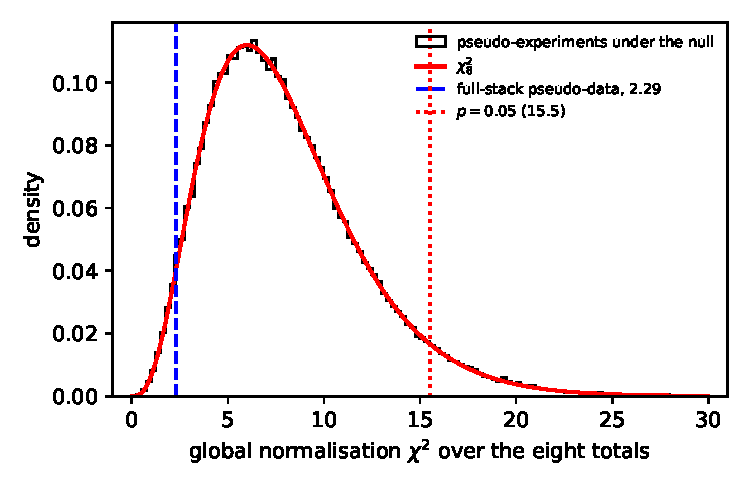
\includegraphics[width=0.85\textwidth]{cr_null_calibration}\\
  \scriptsize\raggedright
  \begin{itemize}\setlength\itemsep{1pt}
    \item Full-stack pseudo-data: global $\chi^2=0.66/8$, 16 pulls within $\pm0.5$, 22 shape tests $p>0.47$.
    \item Power: one region off by $>12\%$ (CC$0\pi$, $\pi^0$) or $>50$--$62\%$ (multi-$\pi$, cosmic) fails;
      a common shift only beyond $58\%$ (absorbed by flux and xsec terms).
    \item Signal held at the tune: a $30\%$ excess moves CC$0\pi$ by $2.8\%$, inside every pull resolution.
  \end{itemize}
  \end{columns}
\end{frame}

\begin{frame}{Backup: control-region distributions (pseudo-data)}
  \begin{columns}[T]
  \column{.55\textwidth}
  \centering
  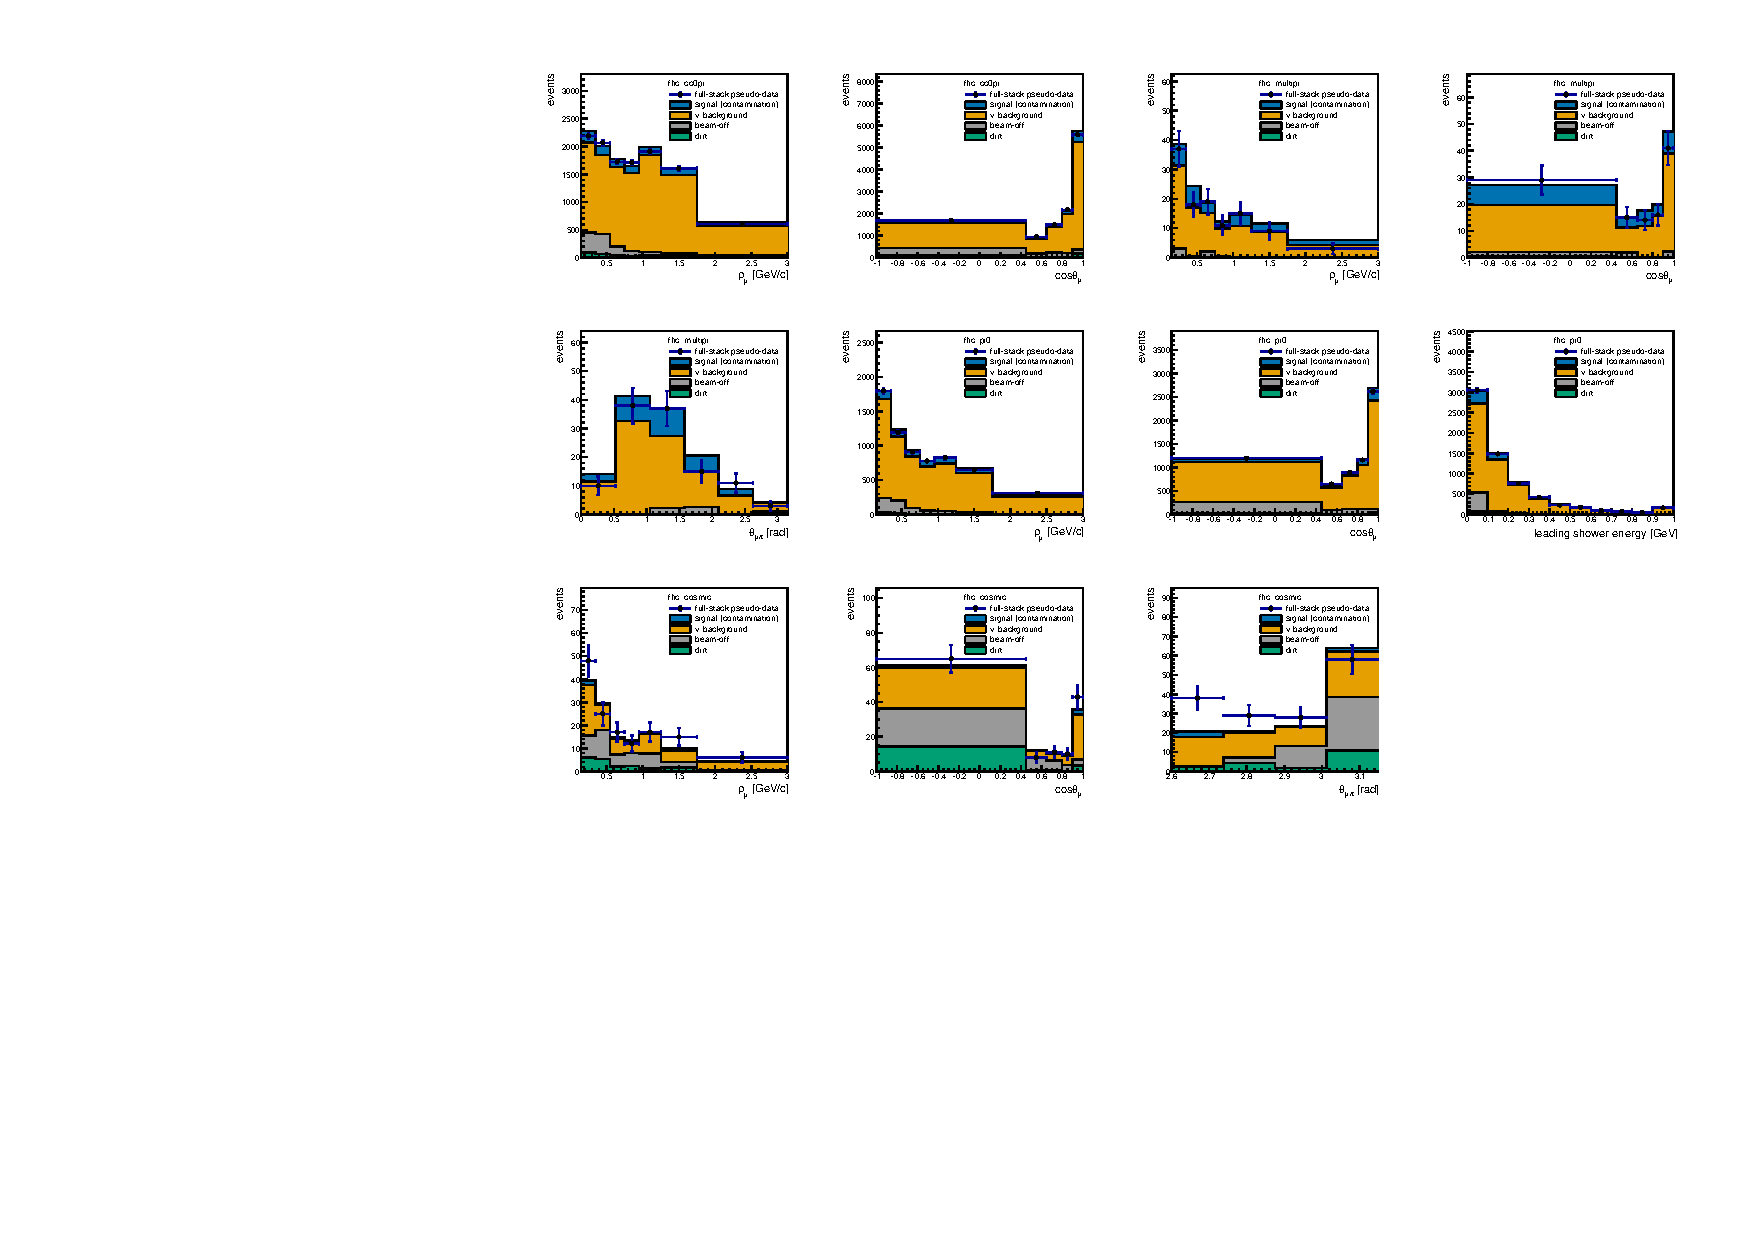
\includegraphics[width=\textwidth]{sideband_plots_fhc}
  \column{.43\textwidth}
  \scriptsize
  \begin{itemize}\setlength\itemsep{3pt}
    \item FHC, frozen binning; rows: CC$0\pi$, multi-$\pi$, $\pi^0$, cosmic.
    \item Points are full-stack pseudo-data ($\nu$ throw plus independent EXT and dirt throws), in place of beam-on.
    \item Data/prediction $0.99$--$1.05$ (FHC), $0.99$--$1.12$ (RHC), $0.99$--$1.08$ (comb.), within statistics.
    \item Tests the bookkeeping path of beam-on data, not the background model.
    \item Regions overlap only between multi-$\pi$ and $\pi^0$ ($38$--$43\%$ of multi-$\pi$).
    \item $\pi^0$ region without the final multiplicity cut: $11$--$14\%$ more events, purity and shape unchanged.
  \end{itemize}
  \end{columns}
\end{frame}

\begin{frame}{Backup: reconstructed spectra and resolution (FHC)}
  \centering
  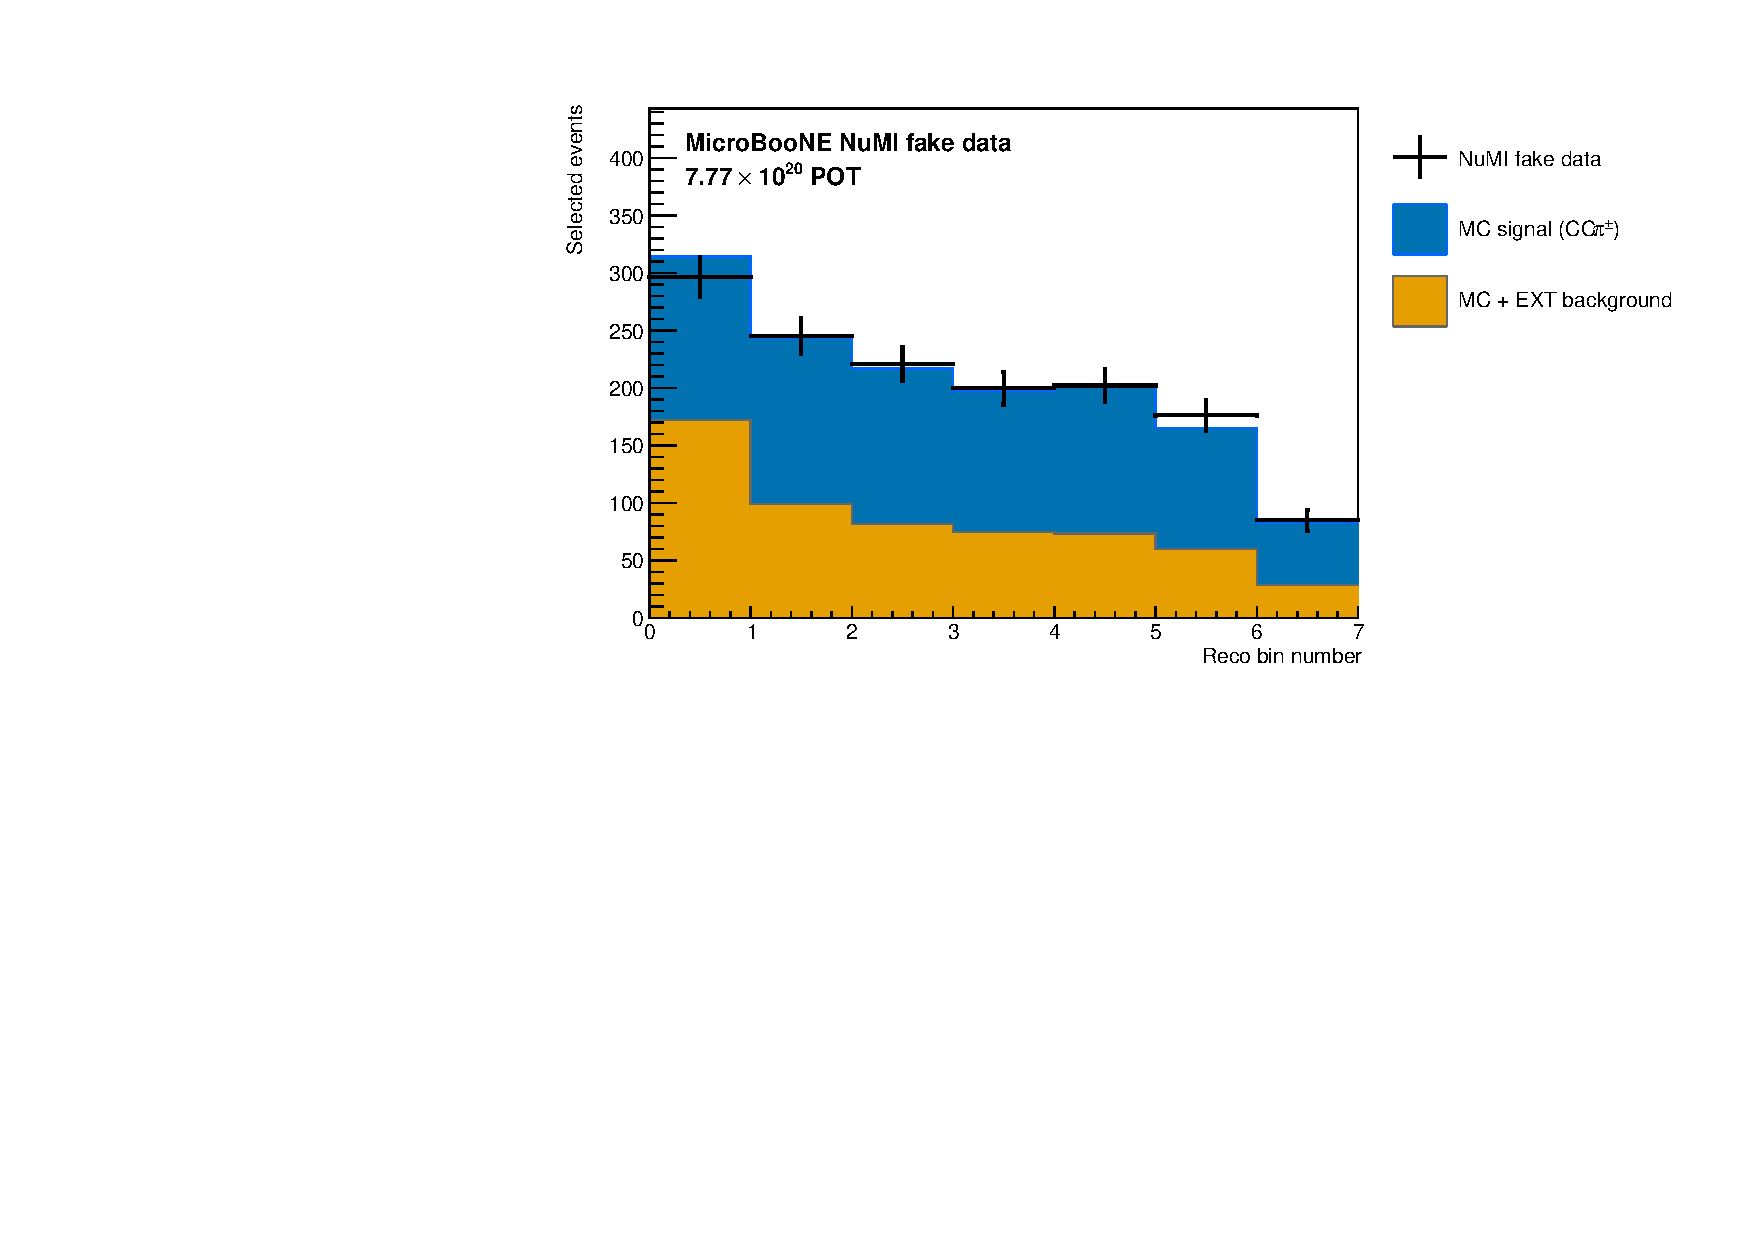
\includegraphics[width=0.24\textwidth]{step1_reco_pmu}\hfill
  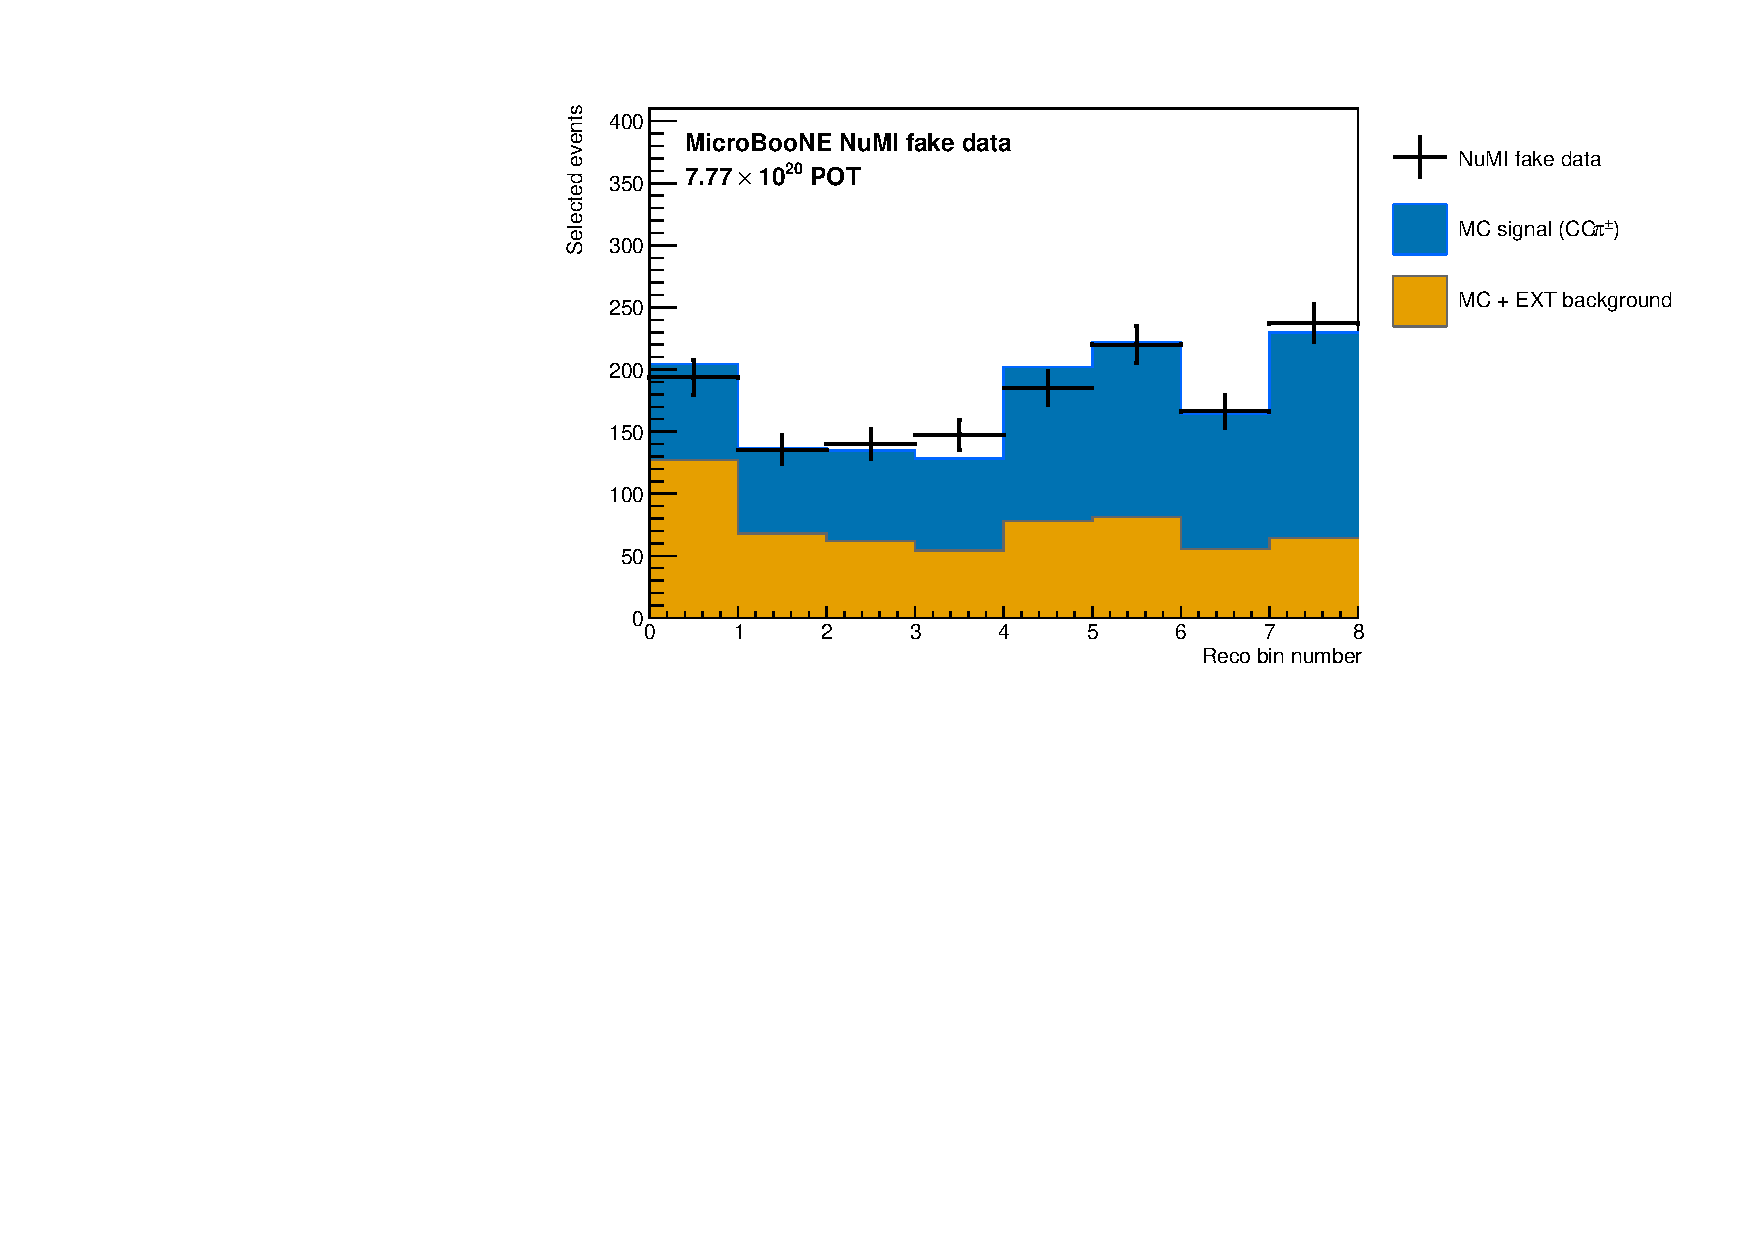
\includegraphics[width=0.24\textwidth]{step1_reco_costhmu}\hfill
  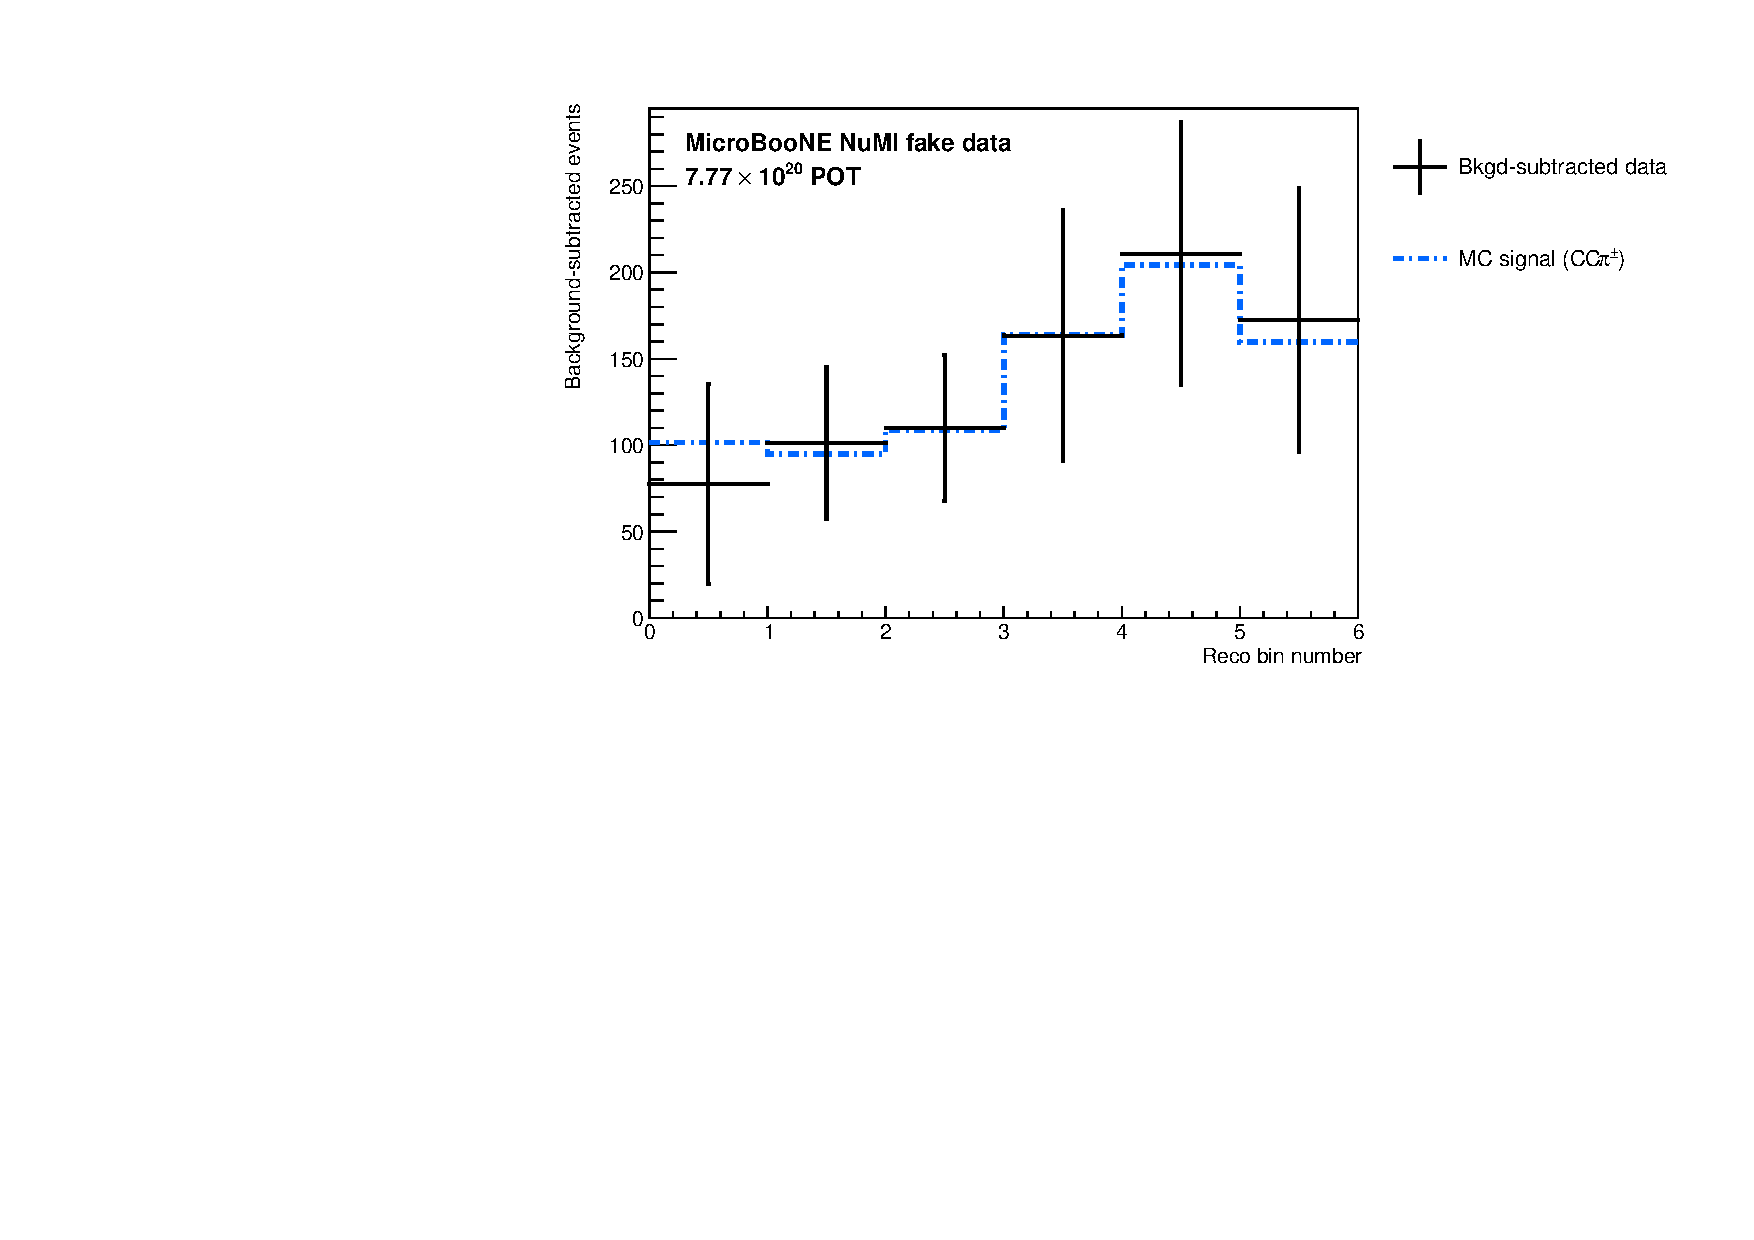
\includegraphics[width=0.24\textwidth]{step2_bsub_pmu}\hfill
  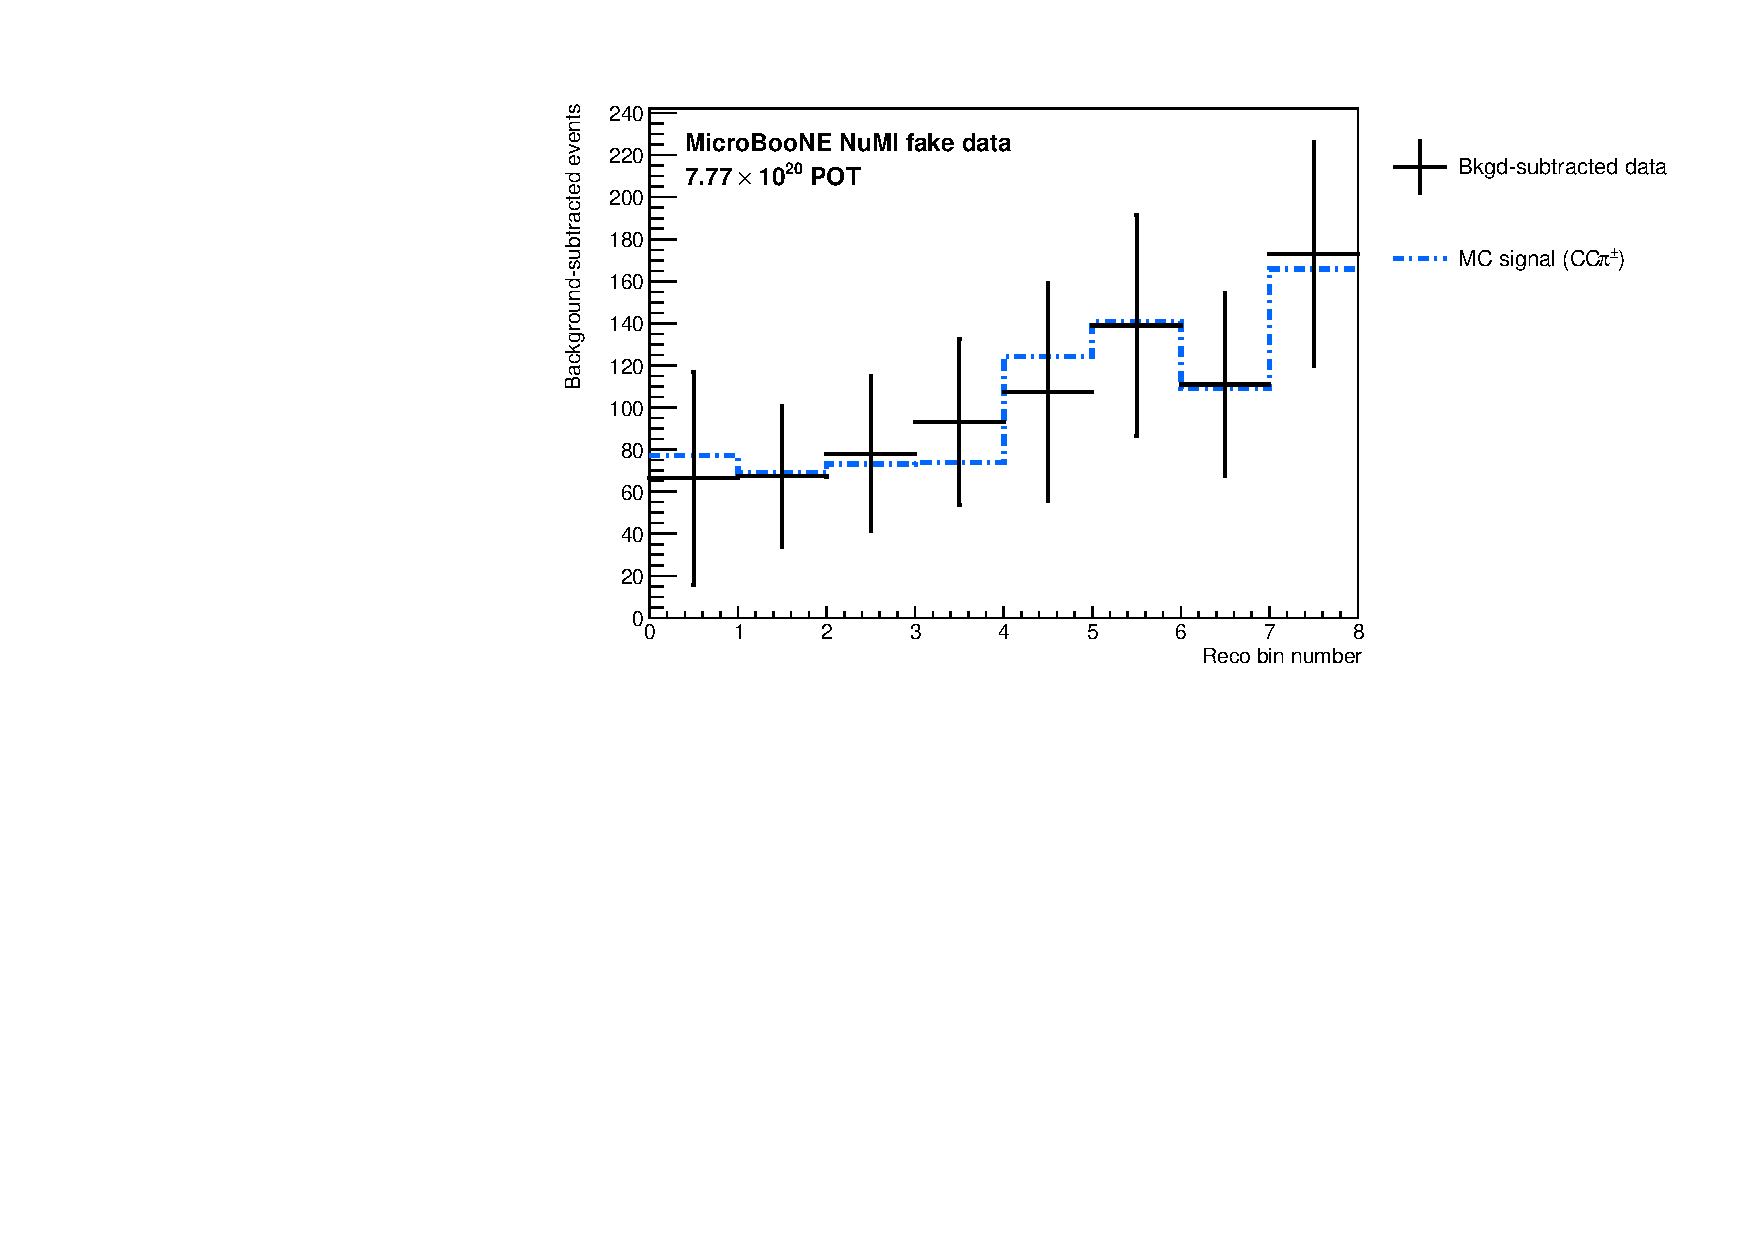
\includegraphics[width=0.24\textwidth]{step2_bsub_costhmu}\\
  {\scriptsize Stage 1 (selected, signal/background split) and stage 2 (background subtracted) for $p_\mu$ and $\cos\theta_\mu$.}\\[1mm]
  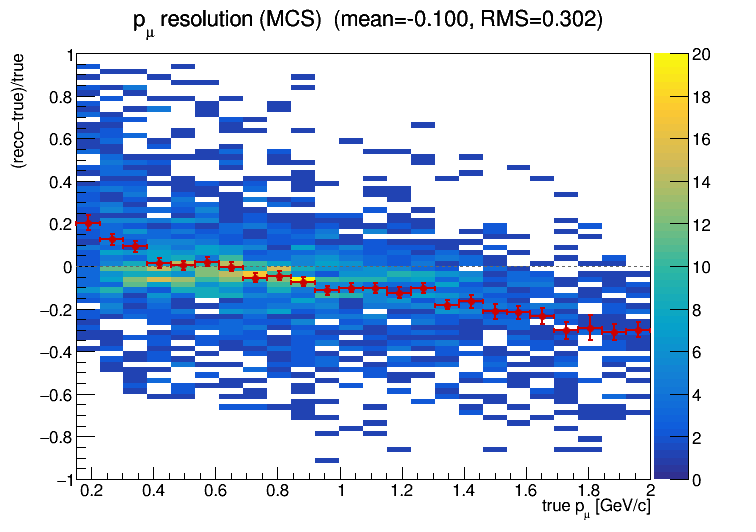
\includegraphics[width=0.24\textwidth]{resolution_pmu_mcs}\hfill
  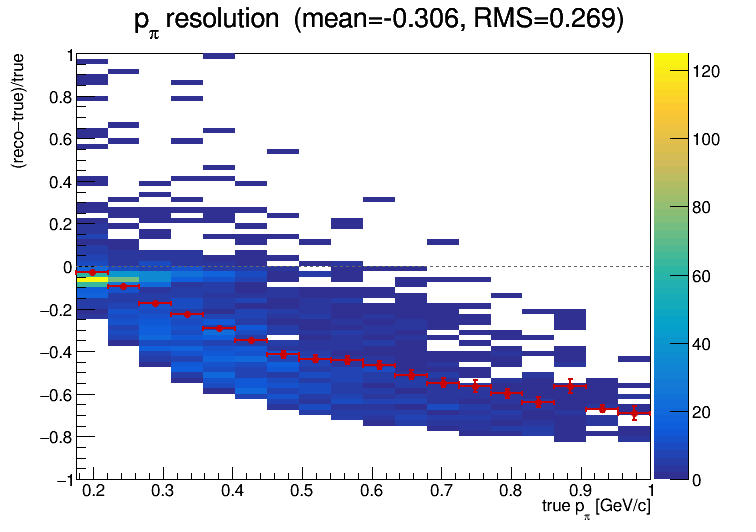
\includegraphics[width=0.24\textwidth]{resolution_ppi}\hfill
  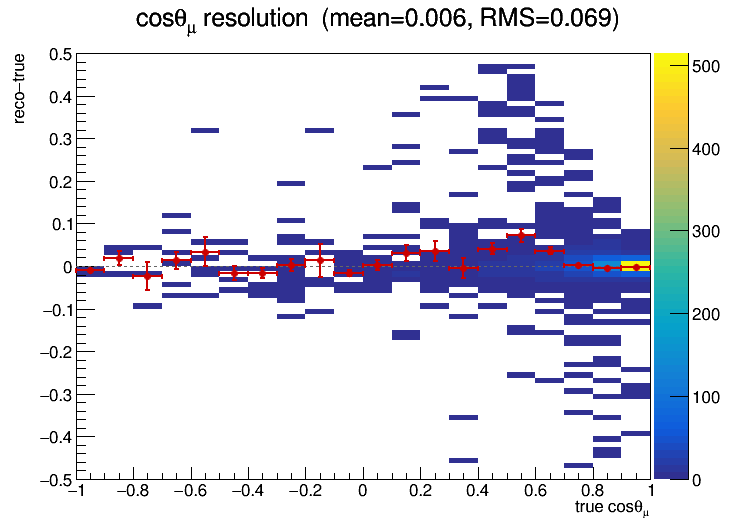
\includegraphics[width=0.24\textwidth]{resolution_costhmu}\hfill
  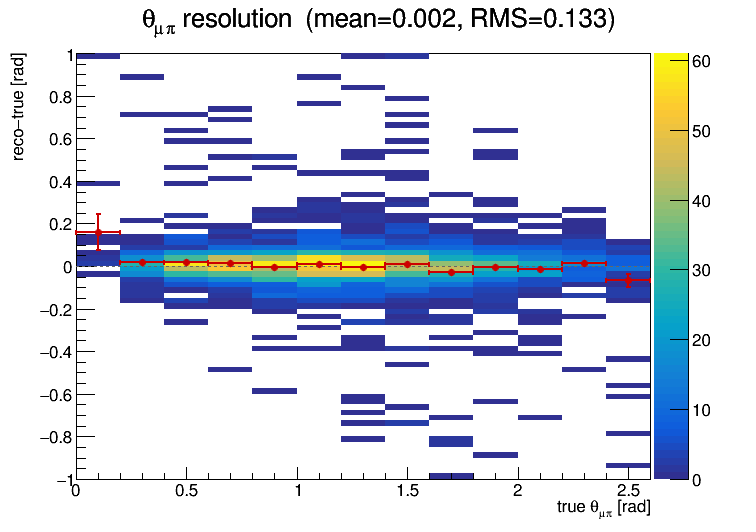
\includegraphics[width=0.24\textwidth]{resolution_thmupi}\\
  {\scriptsize Resolution: $p_\mu$ MCS bias $-9.8\%$, RMS $30\%$; $p_\pi$ bias $-31\%$ (only $-2\%$ in the first bin), RMS $27\%$;
  $\cos\theta_\mu$ RMS $0.076$; $\theta_{\mu\pi}$ RMS $0.135$\,rad.}
\end{frame}

\begin{frame}{Backup: beam-off normalisation per run period}
  \centering
  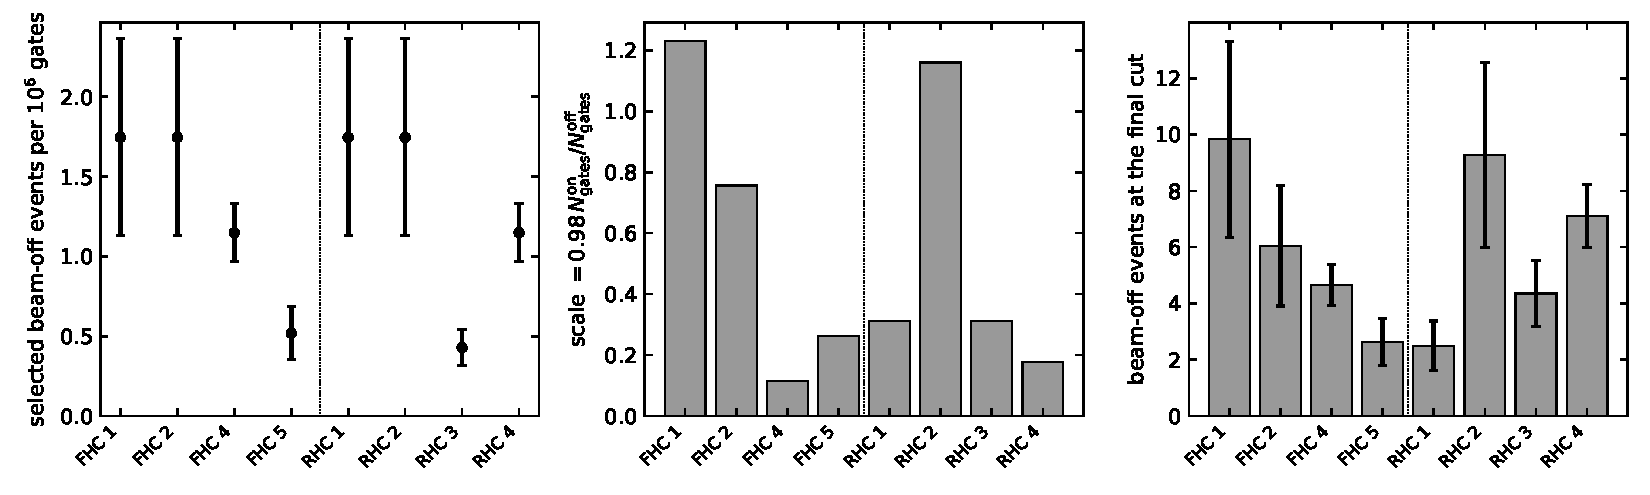
\includegraphics[width=0.95\textwidth]{ext_perrun_validation}\\[2mm]
  \begin{columns}[T]
  \column{.48\textwidth}
  \scriptsize
  \begin{itemize}\setlength\itemsep{1pt}
    \item Rate per $10^6$ triggers at the final cut (left), scale $0.98\times$on/off triggers (centre), events (right).
    \item Run-1 rate is $1.5$--$4\times$ the later periods, so samples are matched by period, not pooled.
  \end{itemize}
  \column{.48\textwidth}
  \scriptsize
  \begin{itemize}\setlength\itemsep{1pt}
    \item Rates from $8$, $14$, $40$, $10$ selected events: Poisson $16$--$35\%$.
    \item Runs 4--5 beam-off use \texttt{swtrig\_pre} (the \texttt{swtrig} flag is zero throughout).
    \item Each (beam-off file, run) pair enters each configuration once.
  \end{itemize}
  \end{columns}
\end{frame}

\begin{frame}{Backup: data release and pipeline}
  \begin{columns}[T]
  \column{.6\textwidth}
  \scriptsize\setlength{\tabcolsep}{3pt}
  \begin{tabular}{@{}p{3.1cm}p{4.9cm}@{}}
    \toprule
    File & Content \\\midrule
    \texttt{curves\_<tag>.tsv} & per bin: edges, width, unfolded data, stat.\ error, truth, tune, generators (all $A_C$-smeared densities) \\
    \texttt{A\_C\_<tag>.tsv} & row $i$ smeared bin, column $j$ true bin; $\mathrm{smeared}_i=\sum_j A_C[i][j]p_j/w_i$ \\
    \texttt{cov/<tag>/cov\_total\_plusMCS.txt} & official covariance \\
    \texttt{cov/<tag>/cov\_<source>.txt} & flux, detector, xsec, re-int., POT, targets, MC, EXT, data, MCS \\
    \texttt{total\_xsec.tsv} & one-bin totals with breakdown \\
    \texttt{index\_extractions.tsv} & every extraction and its status \\
    \bottomrule
  \end{tabular}\\[1mm]
  Tag: \texttt{<incl|1p>\_<FHC5|RHCFULL|COMB>\_<obs>}; 2D: \texttt{incl\_COMB\_costhpi\_costhmu2d}, \texttt{1p\_COMB\_thetap\_dpt2d}.
  \column{.38\textwidth}
  \scriptsize
  \textbf{Reproducibility}
  \begin{itemize}\setlength\itemsep{2pt}
    \item Result set rebuilt from the processed ntuples with empty caches in one pass.
    \item Independent rebuild into a separate tree reproduced every bin of the 51 extractions to $10^{-9}$.
    \item Universe cache keyed on the normalisation scheme; normalisation manifest audits flux, POT, $N_\mathrm{Ar}$ and unfolding across all configurations.
    \item Generator curves reproduced from the released $A_C$ to $4\times10^{-8}$ (96 curves).
    \item Source: tag \texttt{v1.6} (34baa99).
  \end{itemize}
  \end{columns}
\end{frame}

\begin{frame}{Backup: rejected alternatives (technical supplement, Part III)}
  \small
  \begin{itemize}\setlength\itemsep{4pt}
    \item \textbf{First binning optimisation}: seven-bin $p_\mu$ failed both criteria (worst diagonal $0.33$);
      five-bin $\cos\theta_\mu$ failed $0.68$ narrowly ($0.67$). Replaced by the binning review.
    \item \textbf{$\theta_\mu$ instead of $\cos\theta_\mu$}: same diagonals, less retained information; rank-1 with the uniform stencil.
    \item \textbf{Pion threshold below $0.175\GeVc$}: resolution $51$--$56\%$, efficiency $2.2\%$, strongly
      model-dependent correction even as one coarse bin.
    \item \textbf{Five-bin $p_\pi$ response}: diagonals $94/37/23/10/6\%$; pile-up into the first reco bin.
    \item \textbf{Golden-pion classifier and other $p_\pi$ estimators}: match the truth ceiling, do not repair the response.
    \item \textbf{Cosmic-direction cuts}: EXT is a data-driven subtraction ($1.6\%$ of the sample); every
      directional or calorimetric variant removes more signal than the $\approx5$-event statistical gain.
    \item \textbf{Six-bin $W_{\pi p}$ and $W_\mathrm{had}$}: below both criteria; not reported / reduced to two regions.
  \end{itemize}
\end{frame}

\end{document}
